\documentclass[conference]{IEEEtran}

\IEEEoverridecommandlockouts
% The preceding line is only needed to identify funding in the first footnote. If that is unneeded, please comment it out.
\usepackage{cite}
\usepackage{amsmath,amssymb,amsfonts}
\usepackage{algorithmic}
\usepackage{graphicx}
\usepackage{textcomp}
\usepackage{xcolor}
\usepackage{capt-of}
\usepackage{cuted} 
\usepackage{float} 
\usepackage{dblfloatfix}
\usepackage{blindtext}
\usepackage{booktabs}
\usepackage{svg}
\usepackage{tikz}
\usepackage{bondgraphs}

\usepackage{lipsum,parskip,booktabs,graphicx,tabulary,tabularx}

\usepackage{subcaption}

\newcommand\MyLogo{%
  
\includegraphics[width=3cm]{logo.png}% Adjust the width as needed
}

\title{Study and development of an ergonomic haptic interface using flexible coils}
\author{
  \textbf{Candidate:} Morgan CASALE\\

  \begin{minipage}[t]{0.4\textwidth}
    \begin{flushleft}
      
      \textbf{Supervisors:}\\
      Alessandro RIZZO (PoliTO)\\
      Domenico PRATTICHIZZO (UniSi)
    \end{flushleft}    
  \end{minipage}
  \hfill
  \begin{minipage}[t]{0.4\textwidth}
    \begin{flushright}
      \textbf{Co-supervisors:}\\
      Tommaso LISINI BALDI (UniSi)\\
      Leonardo FRANCO (UniSi)
    \end{flushright}
  \end{minipage}
}


\usepackage{tikz}    
\begin{document}
\maketitle
\begin{tikzpicture}[remember picture,overlay]
  \node[anchor=north east,inner sep=5pt] at (current page.north east)
  {
\includegraphics[scale=0.05]{logo.png}};
\end{tikzpicture}


\begin{abstract}
    This thesis aims to explore the use of flexible PCB coils in haptic applications to create realistic touch sensations. Current piezo actuators, commonly used for generating vibratory cues, have limitations such as limited low-frequency responses and lack of flexibility, which are crucial for realistic and wearable haptic interfaces. Flexible PCB coils, capable of producing low-frequency vibrations and withstanding bending stresses, offer a potential solution. The thesis will first create a mathematical model of the force transmission chain of a voice actuator-style haptic device created with flexible coils, considering also how the human finger reacts to its stimuli. It will then present the necessary electronics for driving the device and conclude with the design and testing of prototypes to evaluate the technology's potential and limitations.
\end{abstract}

\section{Physic's Model Study}
The haptic device we tried to develop for this thesis is at its heart a \textbf{multi-physical system}, where electrical, magnetic, and mechanical components interact with each other.
Voice coil actuators are characterized by three main components: a \textbf{coil}, a \textbf{magnet}, and a \textbf{membrane}. The coil generates a magnetic field when a \textbf{current flows} through it and by interacting with the magnetic field generated by the magnet, \textbf{creates a force} that moves the membrane. The membrane is then used to \textbf{transmit this force} to the user's finger, which can feel the force as a \textbf{vibration}.
In this section, we will try to create a complete model to explain its behavior using \textbf{bond graphs}.
\begin{figure}[H]
    \centering
    \resizebox{1\linewidth}{!}{
        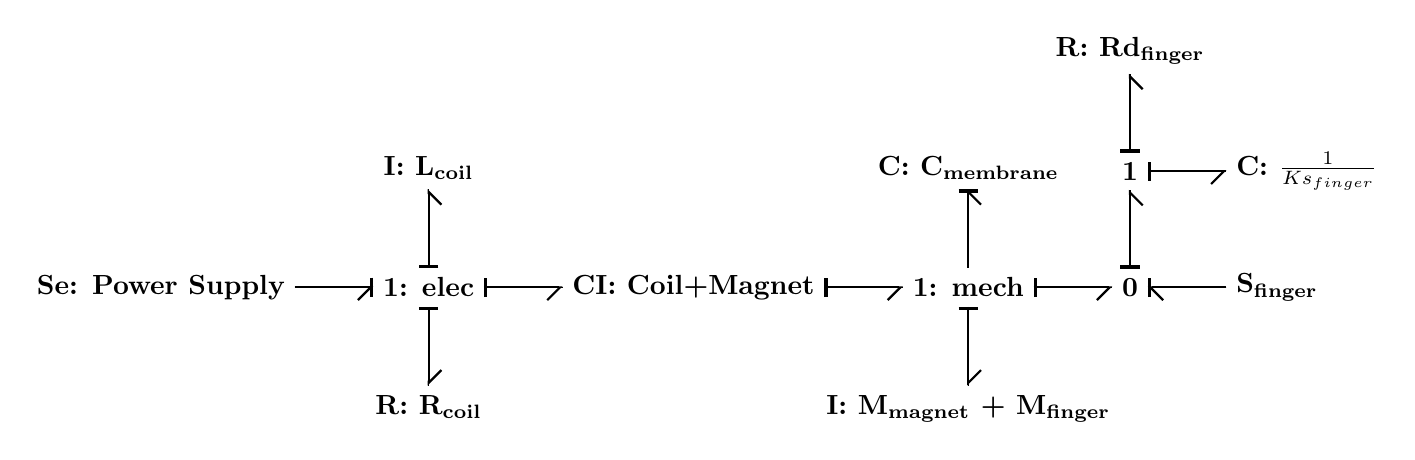
\begin{tikzpicture}
    \begin{scope}[every node/.style={bgelement}]
    \node (Se) at (0,0) {Se: Power Supply};
    \node[right=1 of Se] (i) {1: elec};
    \node[above=1 of i] (Iel) {I: L\textsubscript{coil}};
    \node[below=1 of i] (Rel) {R: R\textsubscript{coil}};
    \node[right=1 of i] (CI) {CI: Coil+Magnet};
    \node[right=1 of CI] (w1) {1: mech};
    \node[above=1 of w1] (Cm) {C: C\textsubscript{membrane}};
    \node[below=1 of w1] (Im) {I: M\textsubscript{magnet} + M\textsubscript{finger}};
    \node[right=1 of w1] (v) {0};
    \node[above=1 of v] (w2) {1};
    \node[above=1 of w2] (Rdf) {R: Rd\textsubscript{finger}};
    \node[right=1 of w2] (Cf) {C: $\frac{1}{Ks_{finger}}$};
    \node[right=1 of v] (Sfa) {S\textsubscript{finger}};
    \end{scope}
    \draw[bonds]
    (Se) edge [e_out] (i)
    (i) edge [e_in] (Iel)
    edge [e_in] (Rel)
    edge [e_in] (CI)
    (CI) edge [e_in] (w1)
    (w1) edge [e_out] (Cm)
    edge [e_in] (Im)
    (w1) edge [e_in] (v)
    (v) edge [e_in] (w2)
    (w2) edge [e_in] (Rdf)
    (w2) edge [e_in] (Cf)
    (Sfa) edge [e_out] (v);
\end{tikzpicture}
    
    } % TODO: Da fare bene
    \caption{Bond graph of the entire system, including the finger.}
    \label{fig: Total_bond-graph}
\end{figure}

\subsection{Electrical and Power Aspects of Coils}
The electrical part consists of the \textbf{voltage power supply} and the coil which is modeled as a \textbf{resistor} and an \textbf{inductor} in series. For this research, we're using planar concentric coils built using \textbf{flexible PCB technology}, this allows us freedom of design in creating a \textbf{flexible actuator}.
Due to their nature, these coils are very thin, which results in \textbf{high resistance} and \textbf{high heat production}. The power flowing through the coil must be \textbf{kept low to avoid damaging it}. This in turn means that the magnetic field generated by the coil will be \textbf{weak}, which can be a problem when trying to create strong haptic feedback.

\subsection{Electro-mechanical Transducer}
The electrical energy is converted into mechanical motion through the \textbf{magnetic repulsion force} between the coil and magnet, so the system acts as a \textbf{transducer}.
\begin{figure}[H]
    \centering
    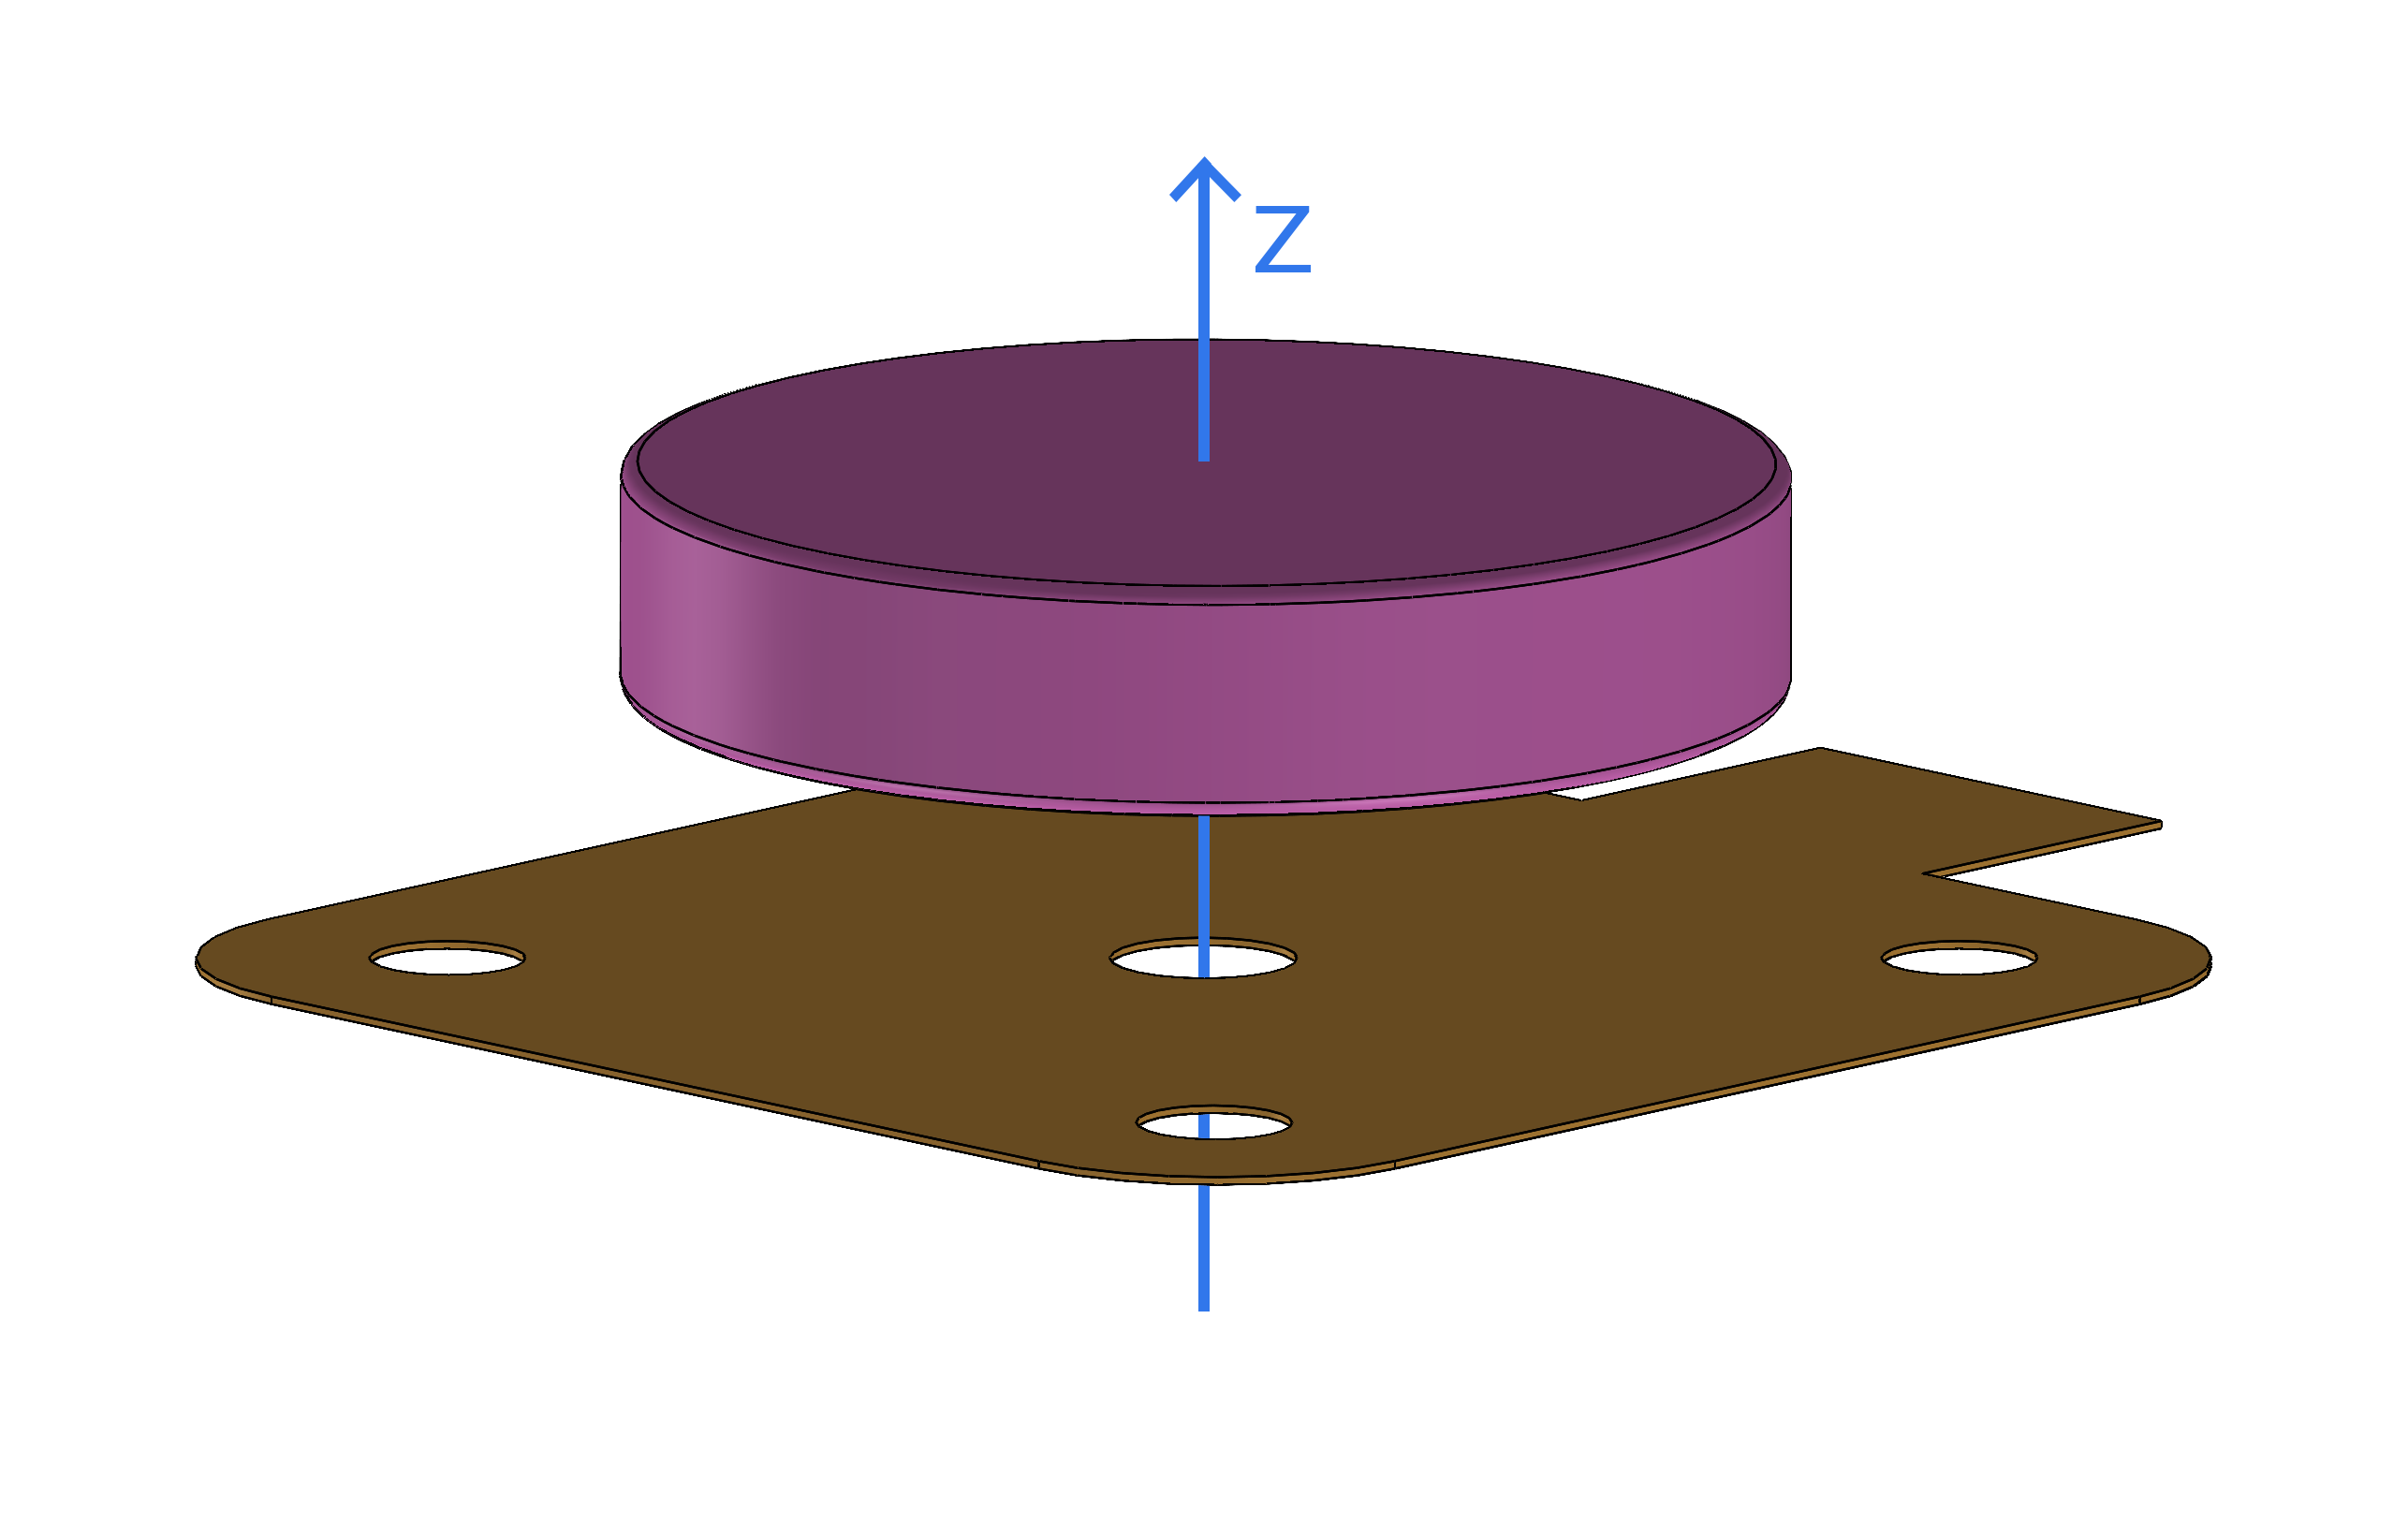
\includegraphics[width=0.4\columnwidth]{Figures/coil_magnet.png} 
    \caption[Coil-Magnet position]{Coil and magnet position in space.}
\end{figure}
The force is calculated through the \textbf{magnetic levitation} equation between the magnetic moment of the magnet and the magnetic field generated by planar windings:
\begin{equation*}
    F = \nabla (\overrightarrow{m_M} \cdot \overrightarrow{B_C}) = \frac{d}{dz} \left( \frac{B_M(z)}{\mu} \cdot \frac{\mu N I R_C^2}{2(R_C^2+z^2)^\frac{3}{2}} \right)
\end{equation*}

\subsection{Mechanical Membrane}
To limit the motion of the magnet only to the z-axis the magnet is inserted in a \textbf{flexible membrane}, this membrane is also used to \textbf{transmit the force} generated by the magnet to the user's finger.
For the last prototype, we designed a \textbf{celtic-cross-shaped silicone membrane} where the magnet is inserted in the center of the cross.
\begin{figure}[H]
    \centering
    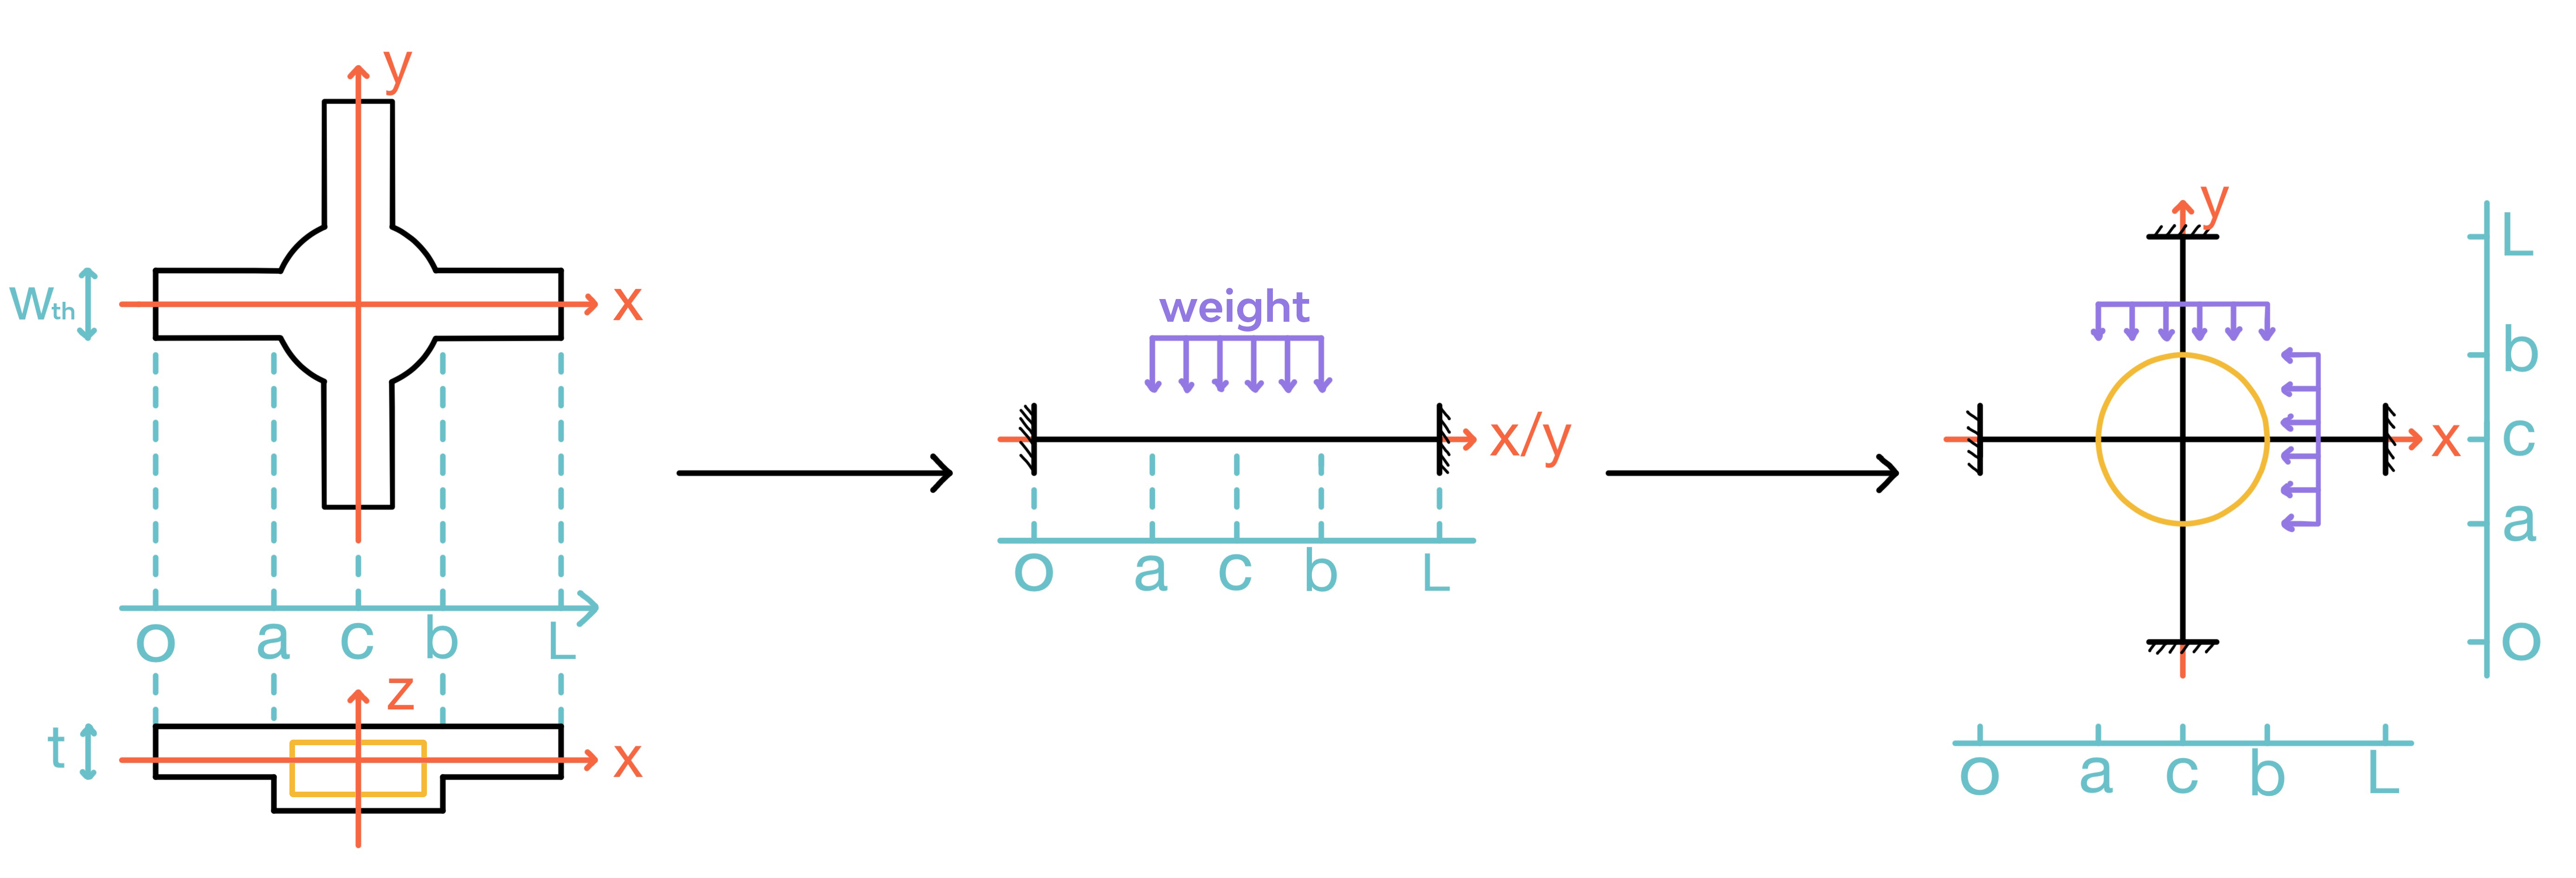
\includegraphics[width=0.9\linewidth]{Figures/membr_mech_model.jpg} 
    \caption[Membrane structure]{Membrane's structure and mechanical model.}
\end{figure}
The membrane can be modeled as a \textbf{spring-damper system}, where the spring represents the stiffness of the membrane, and the damping is negligible.
Finally, the finger grasping the membrane can also be modeled as a \textbf{mass-spring-damper} system where the inertia component is represented by the finger's mass, while the spring and damper represent respectively the stiffness and damping effects of the finger's skin.


\section{Haptics Overview}
Haptic Feedback is the research field that deals with the need to be able to \textbf{digitalize the human sense} of touch and \textbf{reproduce it}.
As this sense is \textbf{very complex} we still don’t understand it fully and we are \textbf{still not able to emulate it completely}. 
The human tactile sensing system can \textbf{measure specific properties of materials}, such as temperature, texture, force, friction, hardness and viscoelasticity, \textbf{through physical contact} between the human skin and the object.
Even the \textbf{changing state of the interaction}, such as gravitational and inertial effects, can be perceived through the sense of touch.
The sense of touch is based on the somatosensory system, which is composed of four main types of receptors, each one is specialized in detecting a specific type of stimulus: \textbf{mechanoreceptors, thermoreceptors, nociceptors and proprioceptors}.
Mechanoreceptors are the most important receptors for haptic feedback, as they are responsible for detecting \textbf{vibration and pressure}.
Their \textbf{sensitivity is limited} in both the frequency and amplitude of vibrations they can detect. The force amplitude limit also depends on the \textbf{constant pressure} applied to the skin.

\section{Device Control Unit}
Using coils to produce magnetic fields of usable intensity requires running them at pretty high currents.
This is because the magnetic field strength is proportional to the current flowing through the coil.
The goal of our device is to generate vibrations at different frequencies so we need to develop an AC-capable power supply.
Standard AC circuits are usually built to generate only low-current signals (in the order of tens of $mA$) but we need to generate signals in the order of $1A$.
For this reason, the control unit we are going to use has in its signal path a power amplifier based on power op-amps. Power op-amps have an integrated power stage that allows them to deliver high currents with a wide frequency bandwidth.
The signal can be generated through a microcontroller with a built-in DAC, in our case we tested the system with an ESP32 board.

\section{Implementation and Prototypes}
\subsection{Rigid Prototype}
The first prototype was designed to test the capabilities of coils produced by the \textbf{HZDR research group}.
In the previous research done by the HZDR team, they tested the coil using a simple piece of \textbf{flexible magnetic tape} as a membrane and magnet.
This membrane is shaped like a "fish" so the tail can be fixed on a plane and the head can be free to bend up and down.
\begin{figure}[H]
    \centering
    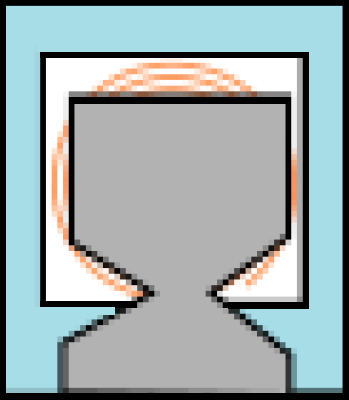
\includegraphics[width = 0.2\linewidth]{Figures/Dresden_test.png}
    \caption{Dresden coil HZDR test setup}
    \label{fig: Dresden_test}
\end{figure}
The pulp needed to be \textbf{suspended} at a certain distance to avoid pressing and stopping the membrane.

To solve this problem we developed a structure able to fulfill this requirement.
\begin{figure}[H]
    \centering
    \begin{subcaptiongroup}
      \centering
      \parbox[b]{0.2\textwidth}{
        \centering
        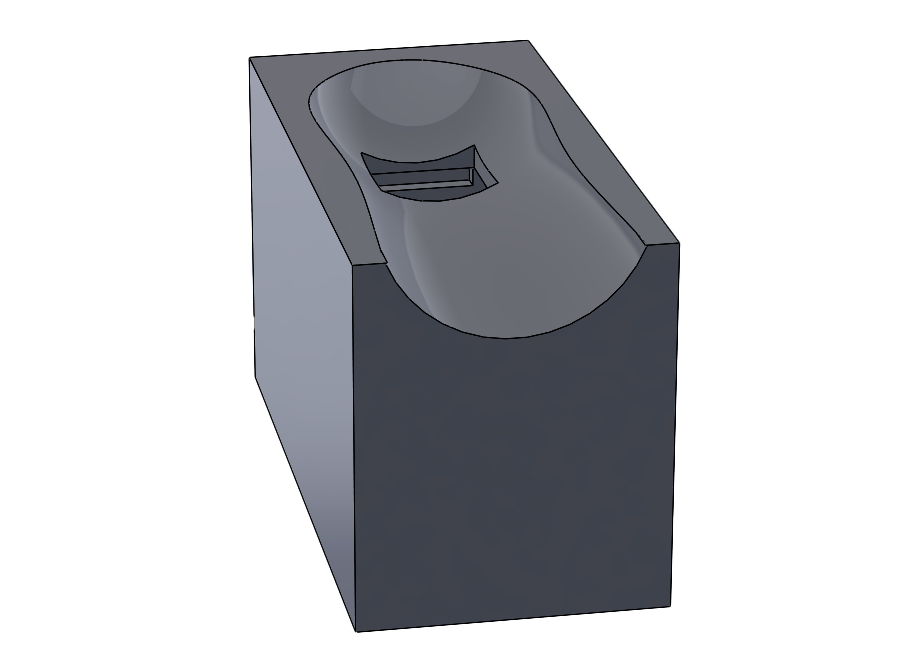
\includegraphics[width = 0.9\linewidth]{Figures/finger_holder.png}
        \caption{Finger resting surface}
      }
      \parbox[b]{0.2\textwidth}{
        \centering
        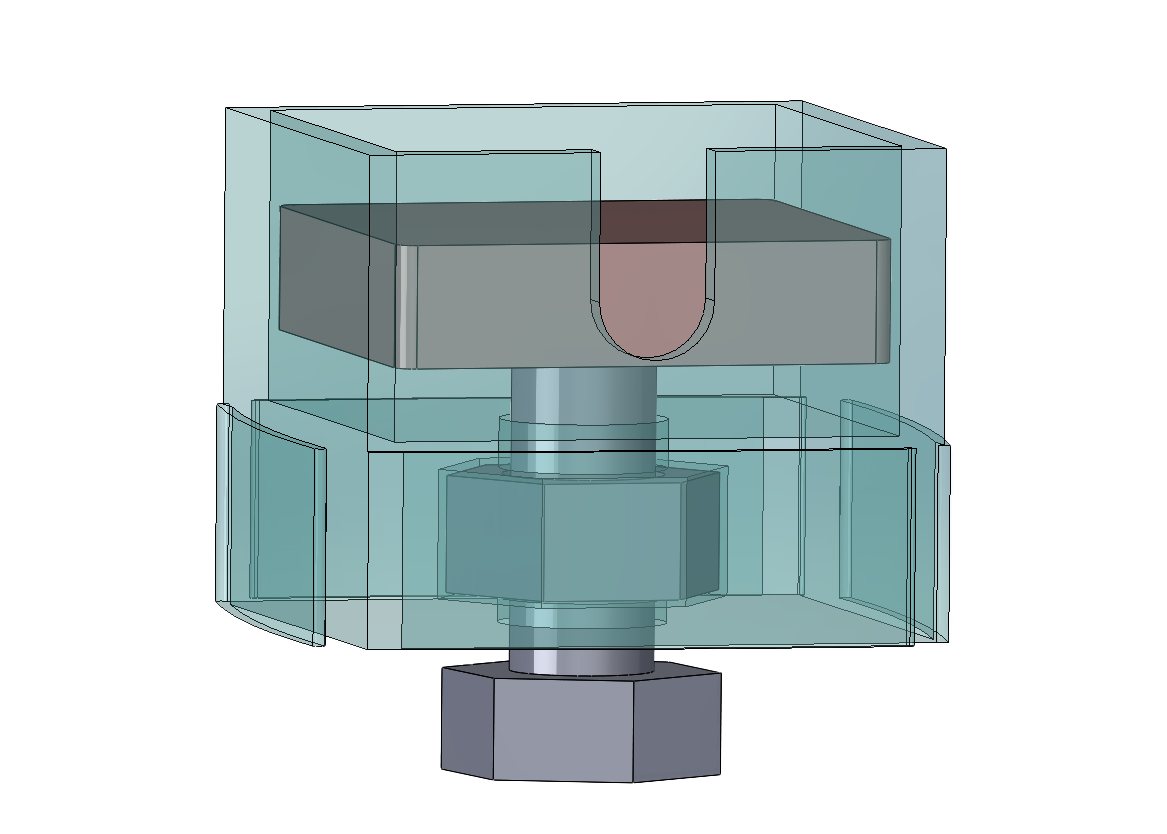
\includegraphics[width = 0.9\linewidth]{Figures/adj_platform.png}
        \caption{Finger platform}
      }
    \end{subcaptiongroup}
    \caption{Components of the first prototype}
\end{figure}
The coil and membrane are placed on top of the \textbf{height-adjustable platform}, to feel the vibrations the finger would lay on the hole of the resting surface.
We quickly moved on from this prototype as the coil was not able to generate \textbf{enough force} to be felt by the user because its \textbf{low power rating} limited its capability to generate a \textbf{strong enough magnetic field}.

\subsection{Wearable Rigid Prototype}
The following prototype was based on the flexible PCB coils. 
These have a \textbf{higher power rating}, can be \textbf{easily designed and manufactured} and are \textbf{sturdier} than the previous ones, especially under flexing conditions. 
A structure was designed to keep the coil in place and allow it to be \textbf{worn on the finger} through the use of silicon sleeves.
This sleeve was designed to be \textbf{adaptable to different finger sizes} and to \textbf{integrate a cylindrical magnet} on the pulp.
\begin{figure}[H]
    \centering
    \begin{subcaptiongroup}
        \centering
        \parbox[b]{0.2\textwidth}{
            \centering
            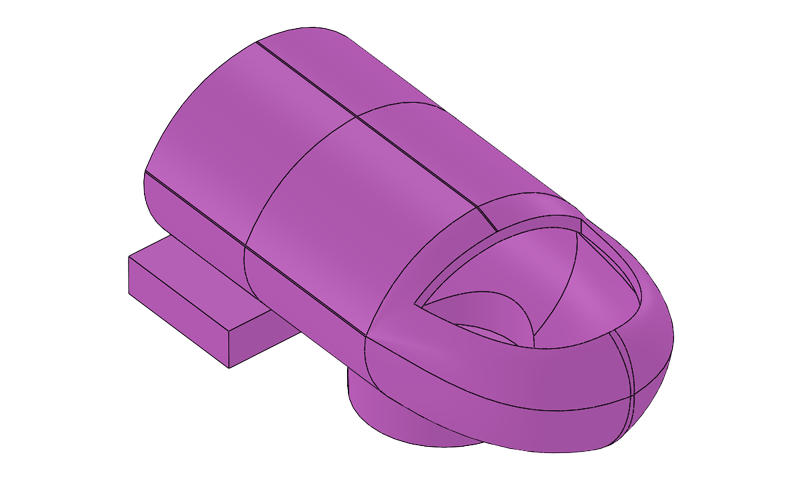
\includegraphics[width=0.2\textwidth]{Figures/silicon_sleeve_front.png}
        }
        \parbox[b]{0.2\textwidth}{
            \centering
            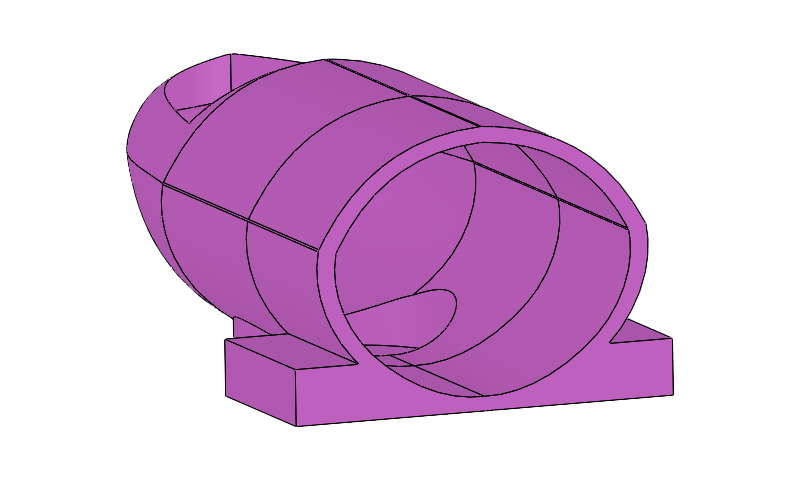
\includegraphics[width=0.2\textwidth]{Figures/silicon_sleeve_back.png}        
        }
    \end{subcaptiongroup}
    \caption{Finger silicon sleeve front and back view}
\end{figure}
The silicon sleeve could be then connected to the assembly where the coil and a heatsink were placed through its lateral mounting wings.
\begin{figure}[H]
    \centering
    \begin{subcaptiongroup}
        \centering
        \parbox[b]{0.2\textwidth}{
            \centering
            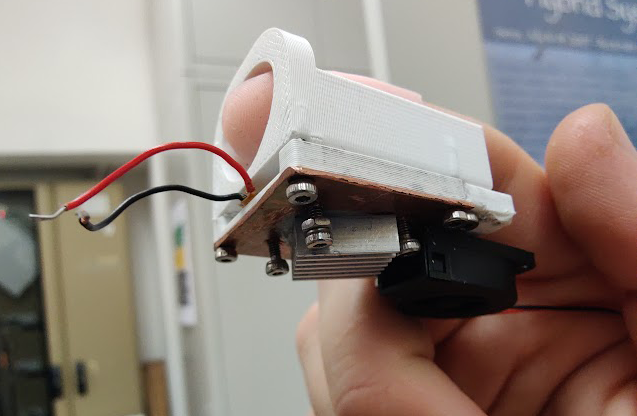
\includegraphics[width=0.2\textwidth]{Figures/rigid_prot_btm.png}
        }
        \parbox[b]{0.2\textwidth}{
            \centering
            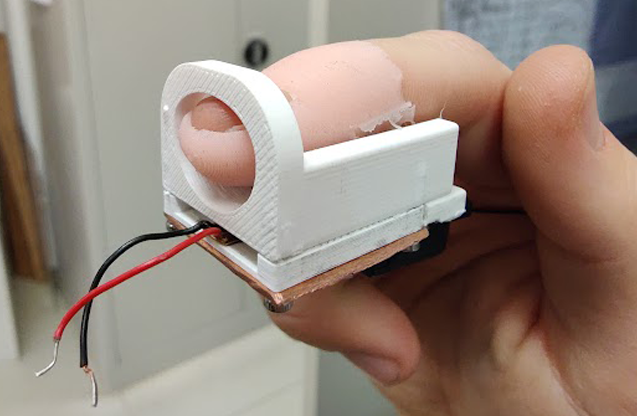
\includegraphics[width=0.2\textwidth]{Figures/rigid_prot_top.png}
        }
    \end{subcaptiongroup}
    \caption{Bottom and top view of the real prototype}
\end{figure}
This prototype is \textbf{much better} than the previous one, the \textbf{magnet} was kept \textbf{at the right distance} from the coil and the vibrations were \textbf{much more noticeable}, also being wearable made it much easier to use.
Its biggest problem was the \textbf{silicon sleeve}, as the silicon tends to \textbf{absorb some of the vibrations} and the softness of the material made the mounting mechanism a bit \textbf{unreliable}.  
We also had to add a small blowing fan to the heatsink to keep the coil cool as it would \textbf{heat a lot} after a few minutes of use.

\subsection{Flexible Mat Prototypes}
The final prototype was designed to be a \textbf{flexible silicon mat where all components were integrated}, including the membrane.

\newsavebox{\largestimage}
\begin{figure}[H]
    \centering
    \savebox{\largestimage}{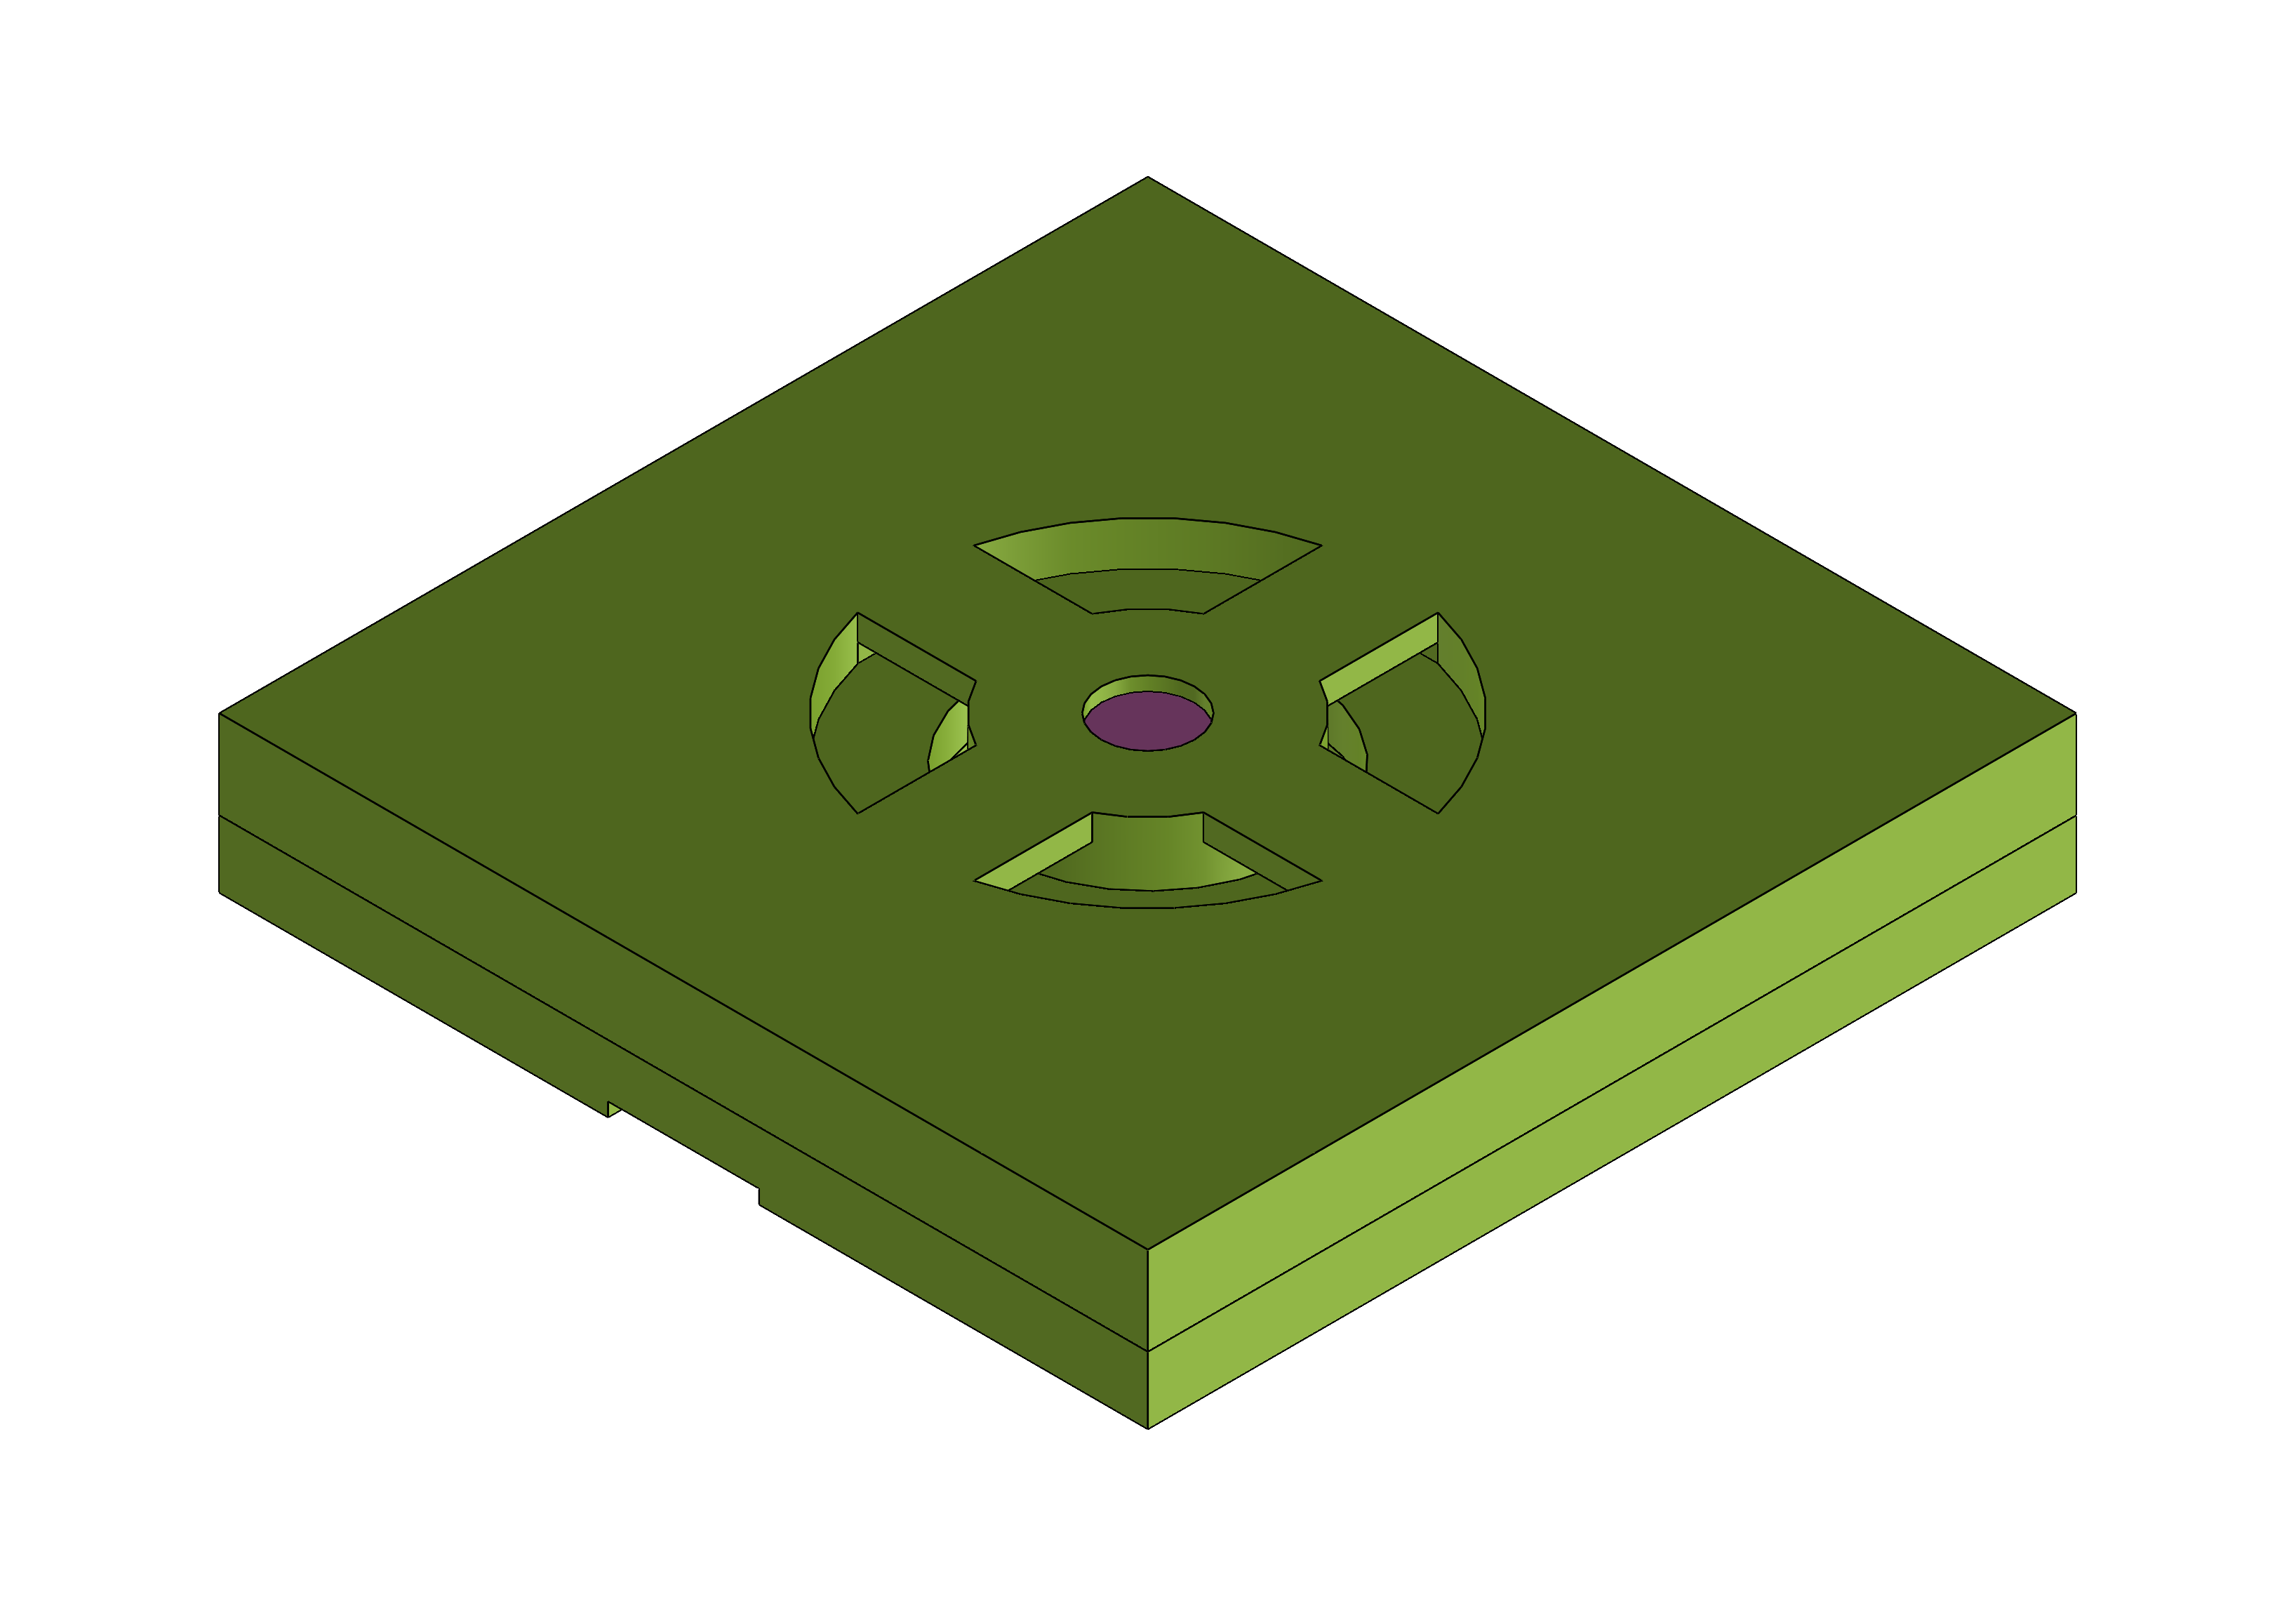
\includegraphics[width=0.2\textwidth]{Figures/membrane_v1.png}}
    \begin{subcaptiongroup}
        \centering
        \parbox[b]{0.2\textwidth}{
            \centering
            \usebox{
                \largestimage
            }
        }
        \parbox[b]{0.2\textwidth}{
            \centering
            \raisebox{\dimexpr.5\ht\largestimage-.5\height}{
                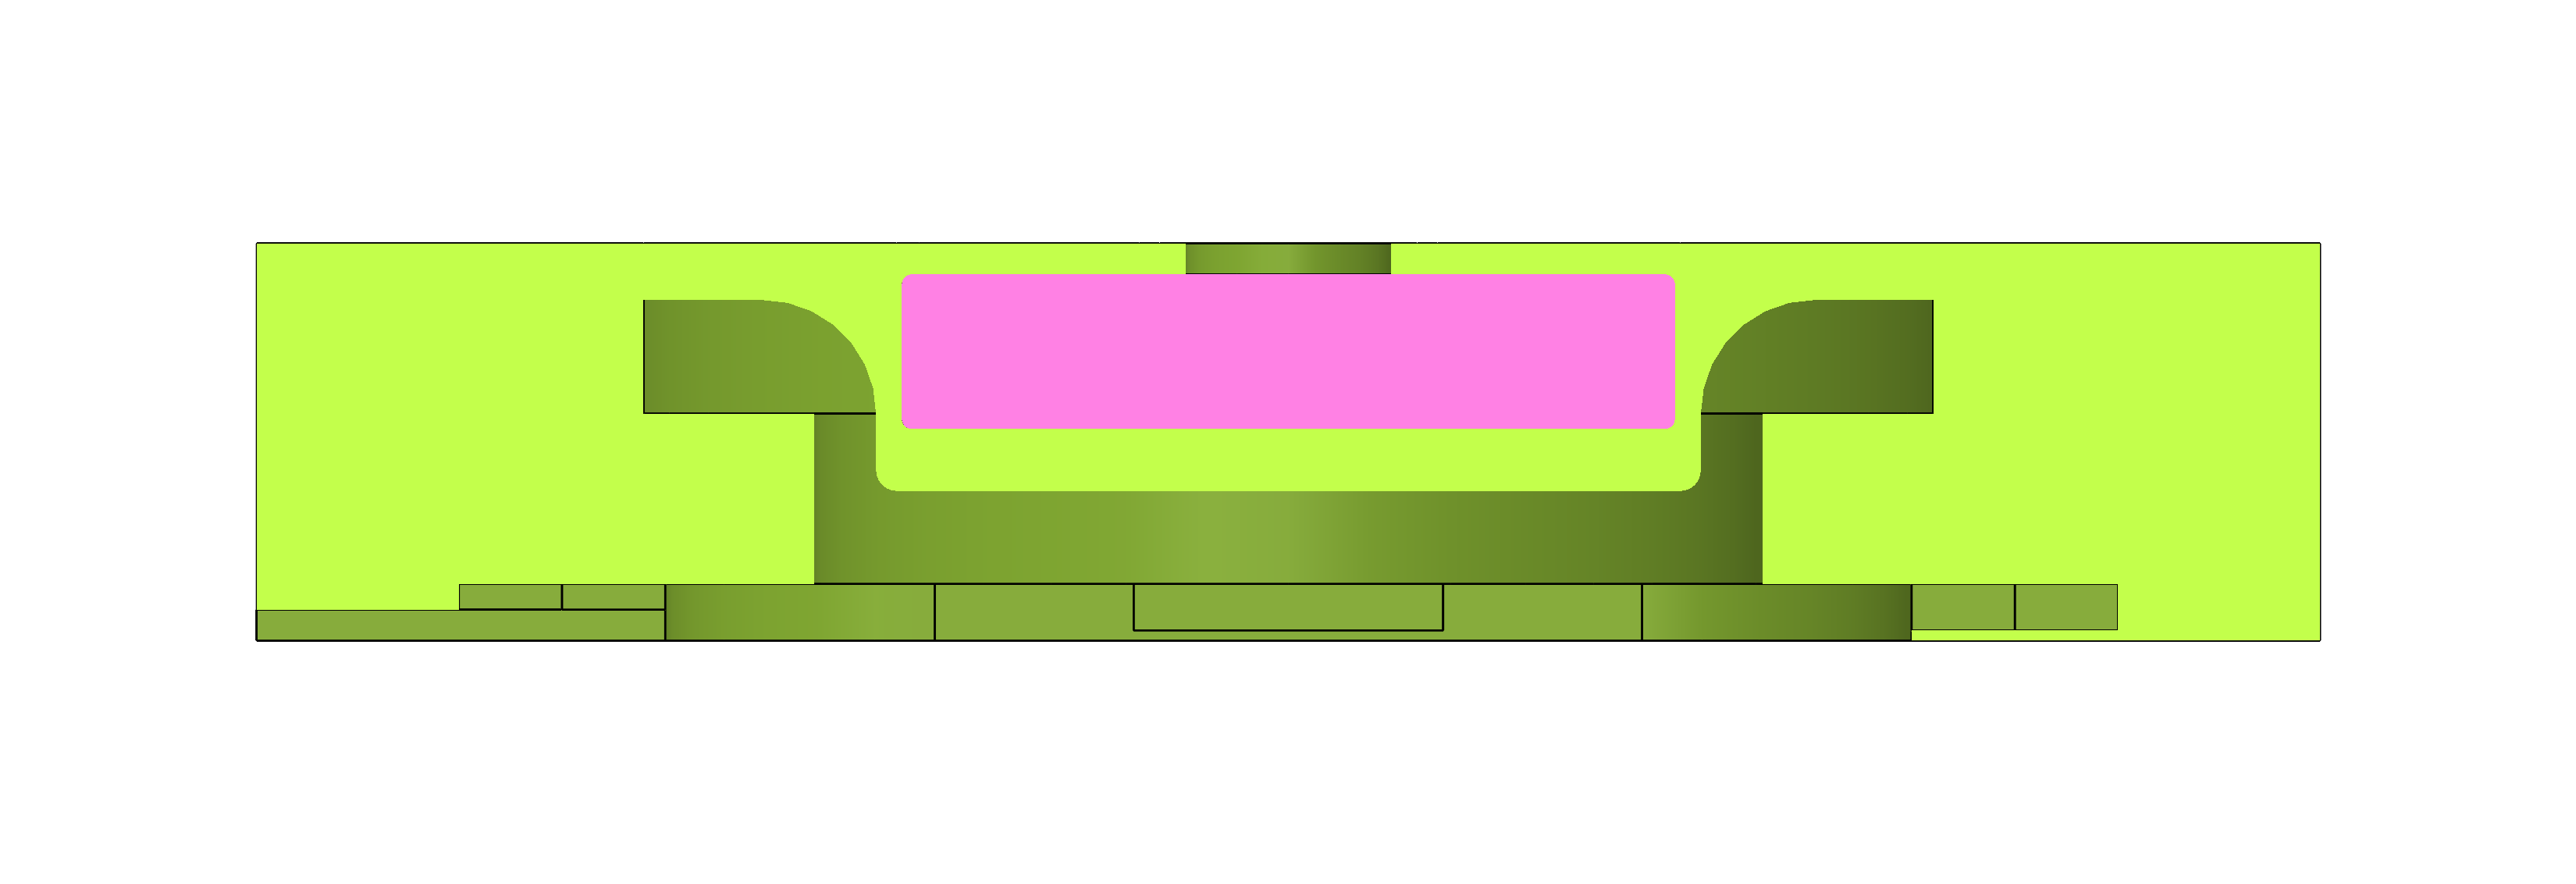
\includegraphics[width=0.2\textwidth]{Figures/membrane_v2_section.png}
            }
        }
    \end{subcaptiongroup}
    \caption{Top and section view of the flexible mat prototype}
\end{figure}
The magnet is suspended inside the silicon membrane and the coil is kept in place at the bottom of the mat.
The coil is kept inside the silicone structure thanks to a \textbf{flexible component} that is in part encased in the silicon and \textbf{acts as a trap}.

\newsavebox{\bigimage}
\begin{figure}[H]
    \centering
    \savebox{\bigimage}{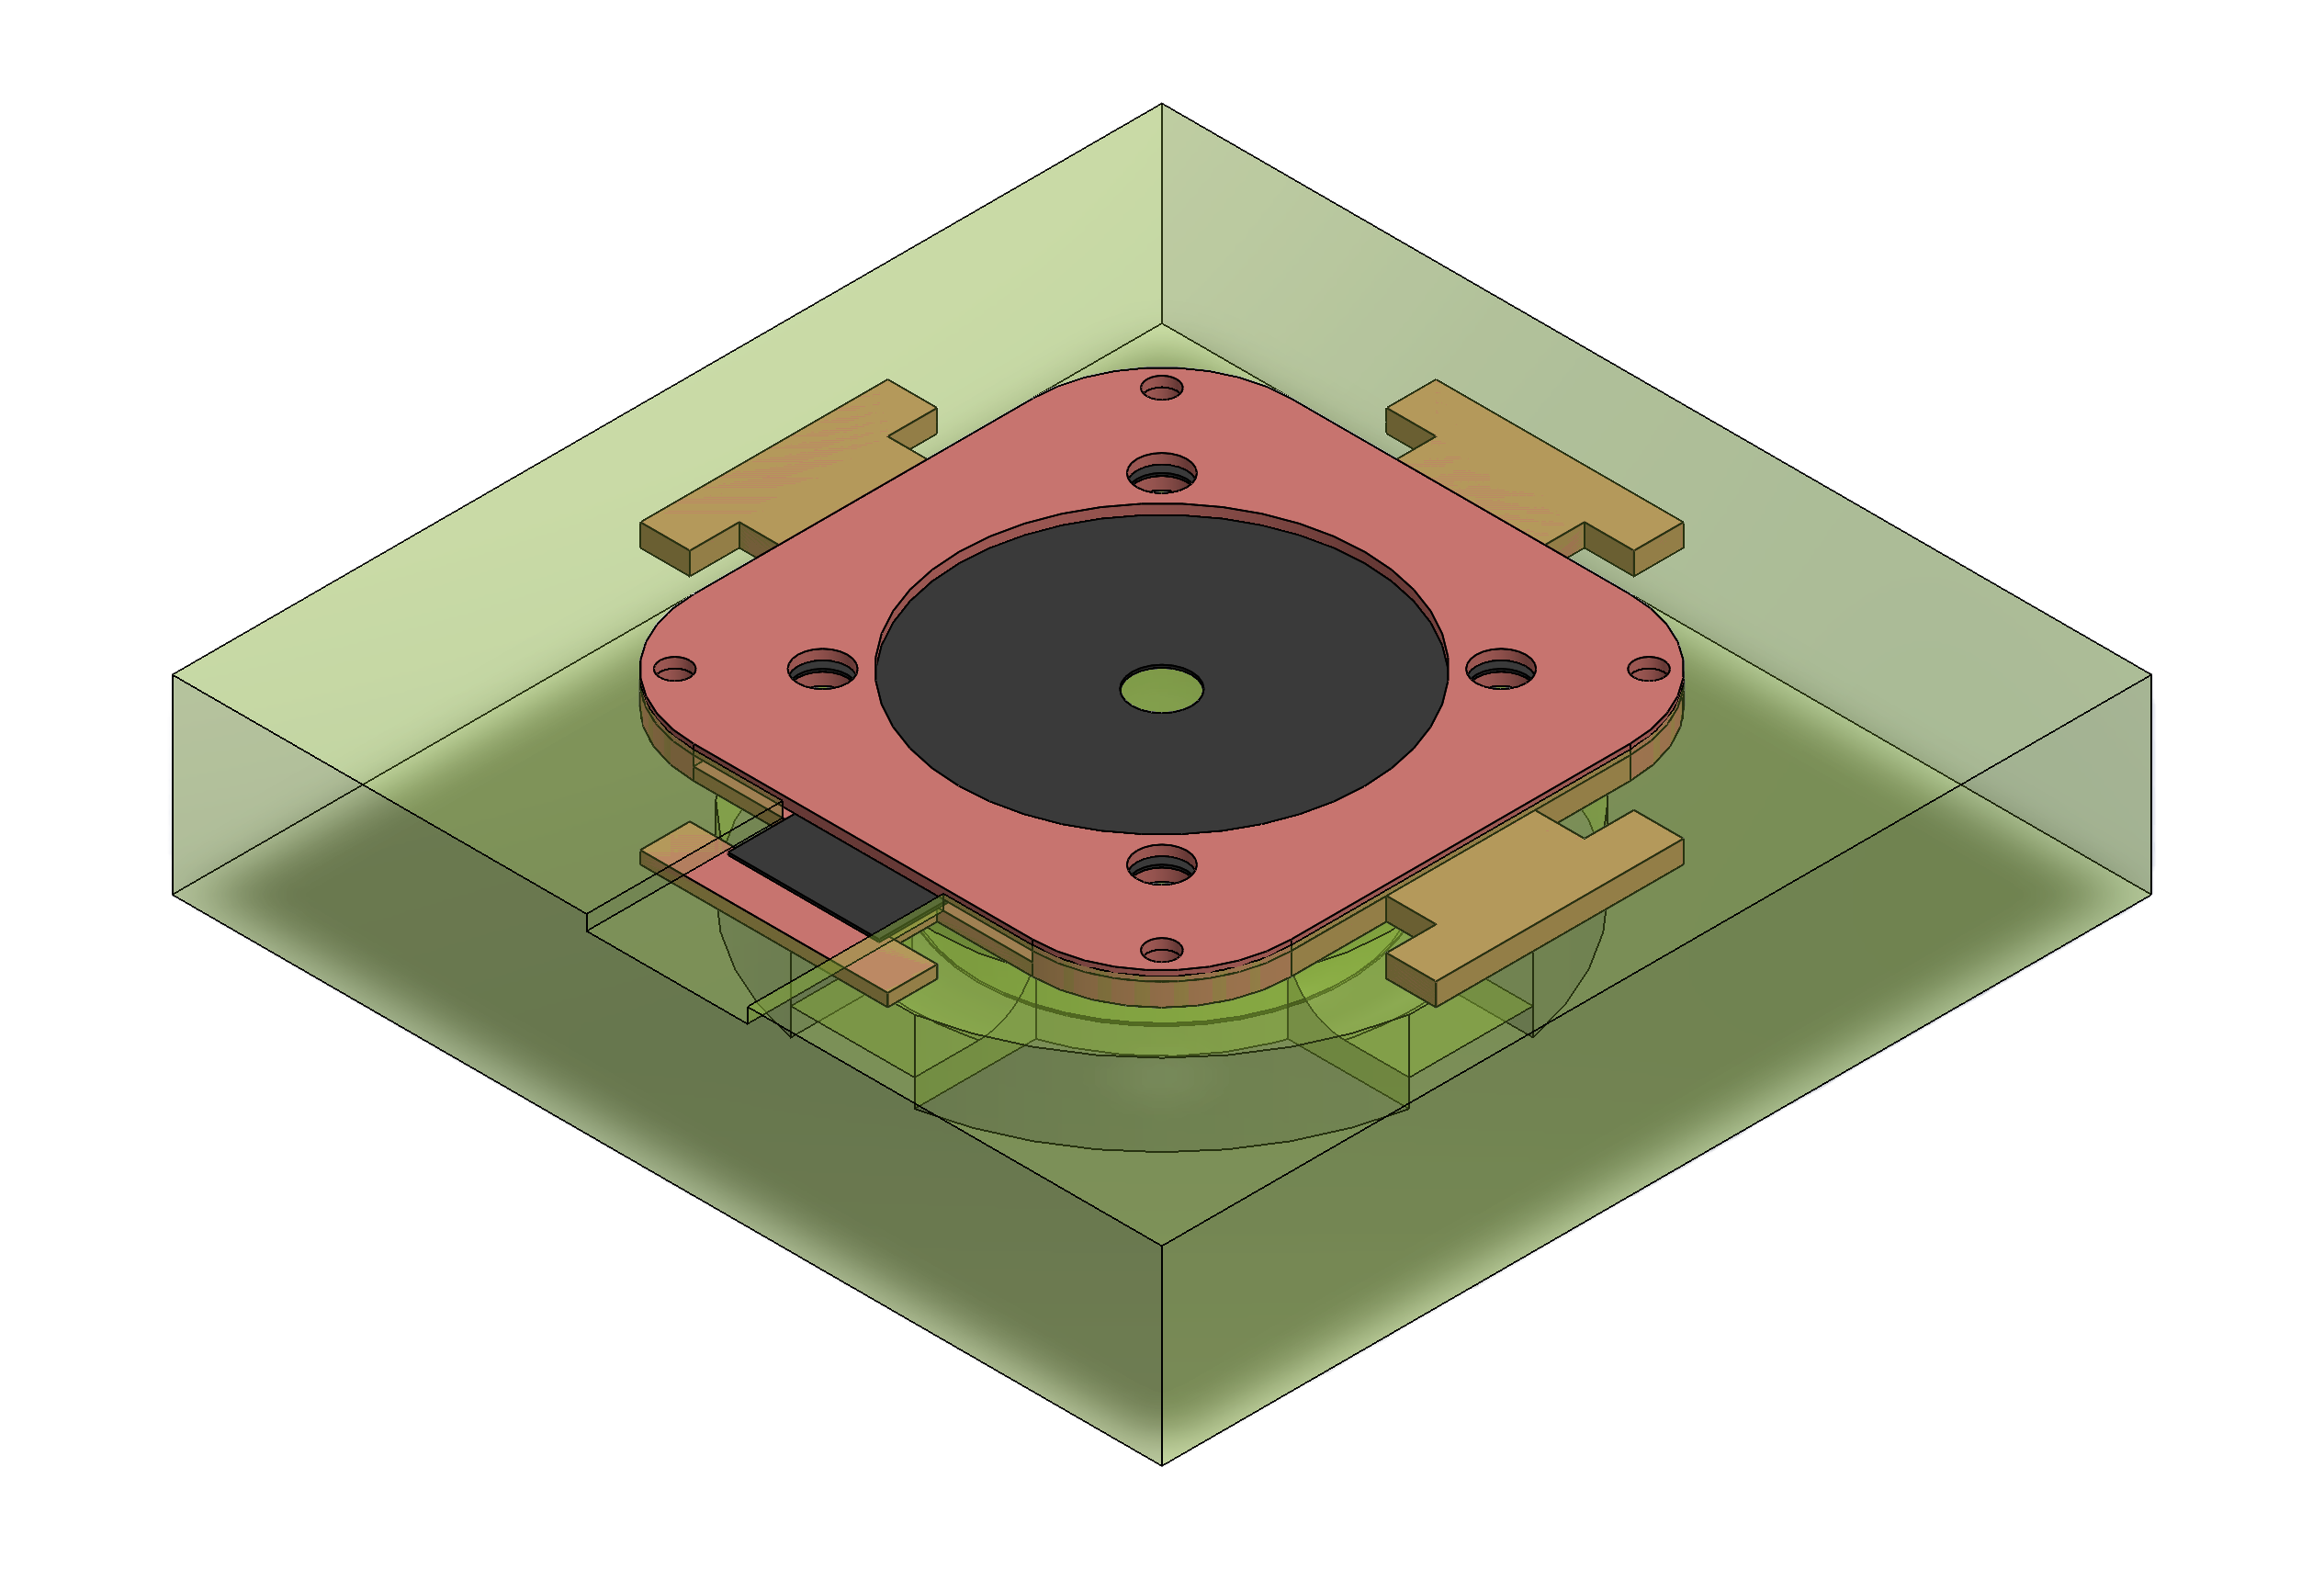
\includegraphics[width=0.2\textwidth]{Figures/coil_trap_in_mat.png}}
    \begin{subcaptiongroup}
        \centering
        \parbox[b]{0.2\textwidth}{
            \centering
            \raisebox{\dimexpr.5\ht\bigimage-.5\height}{
                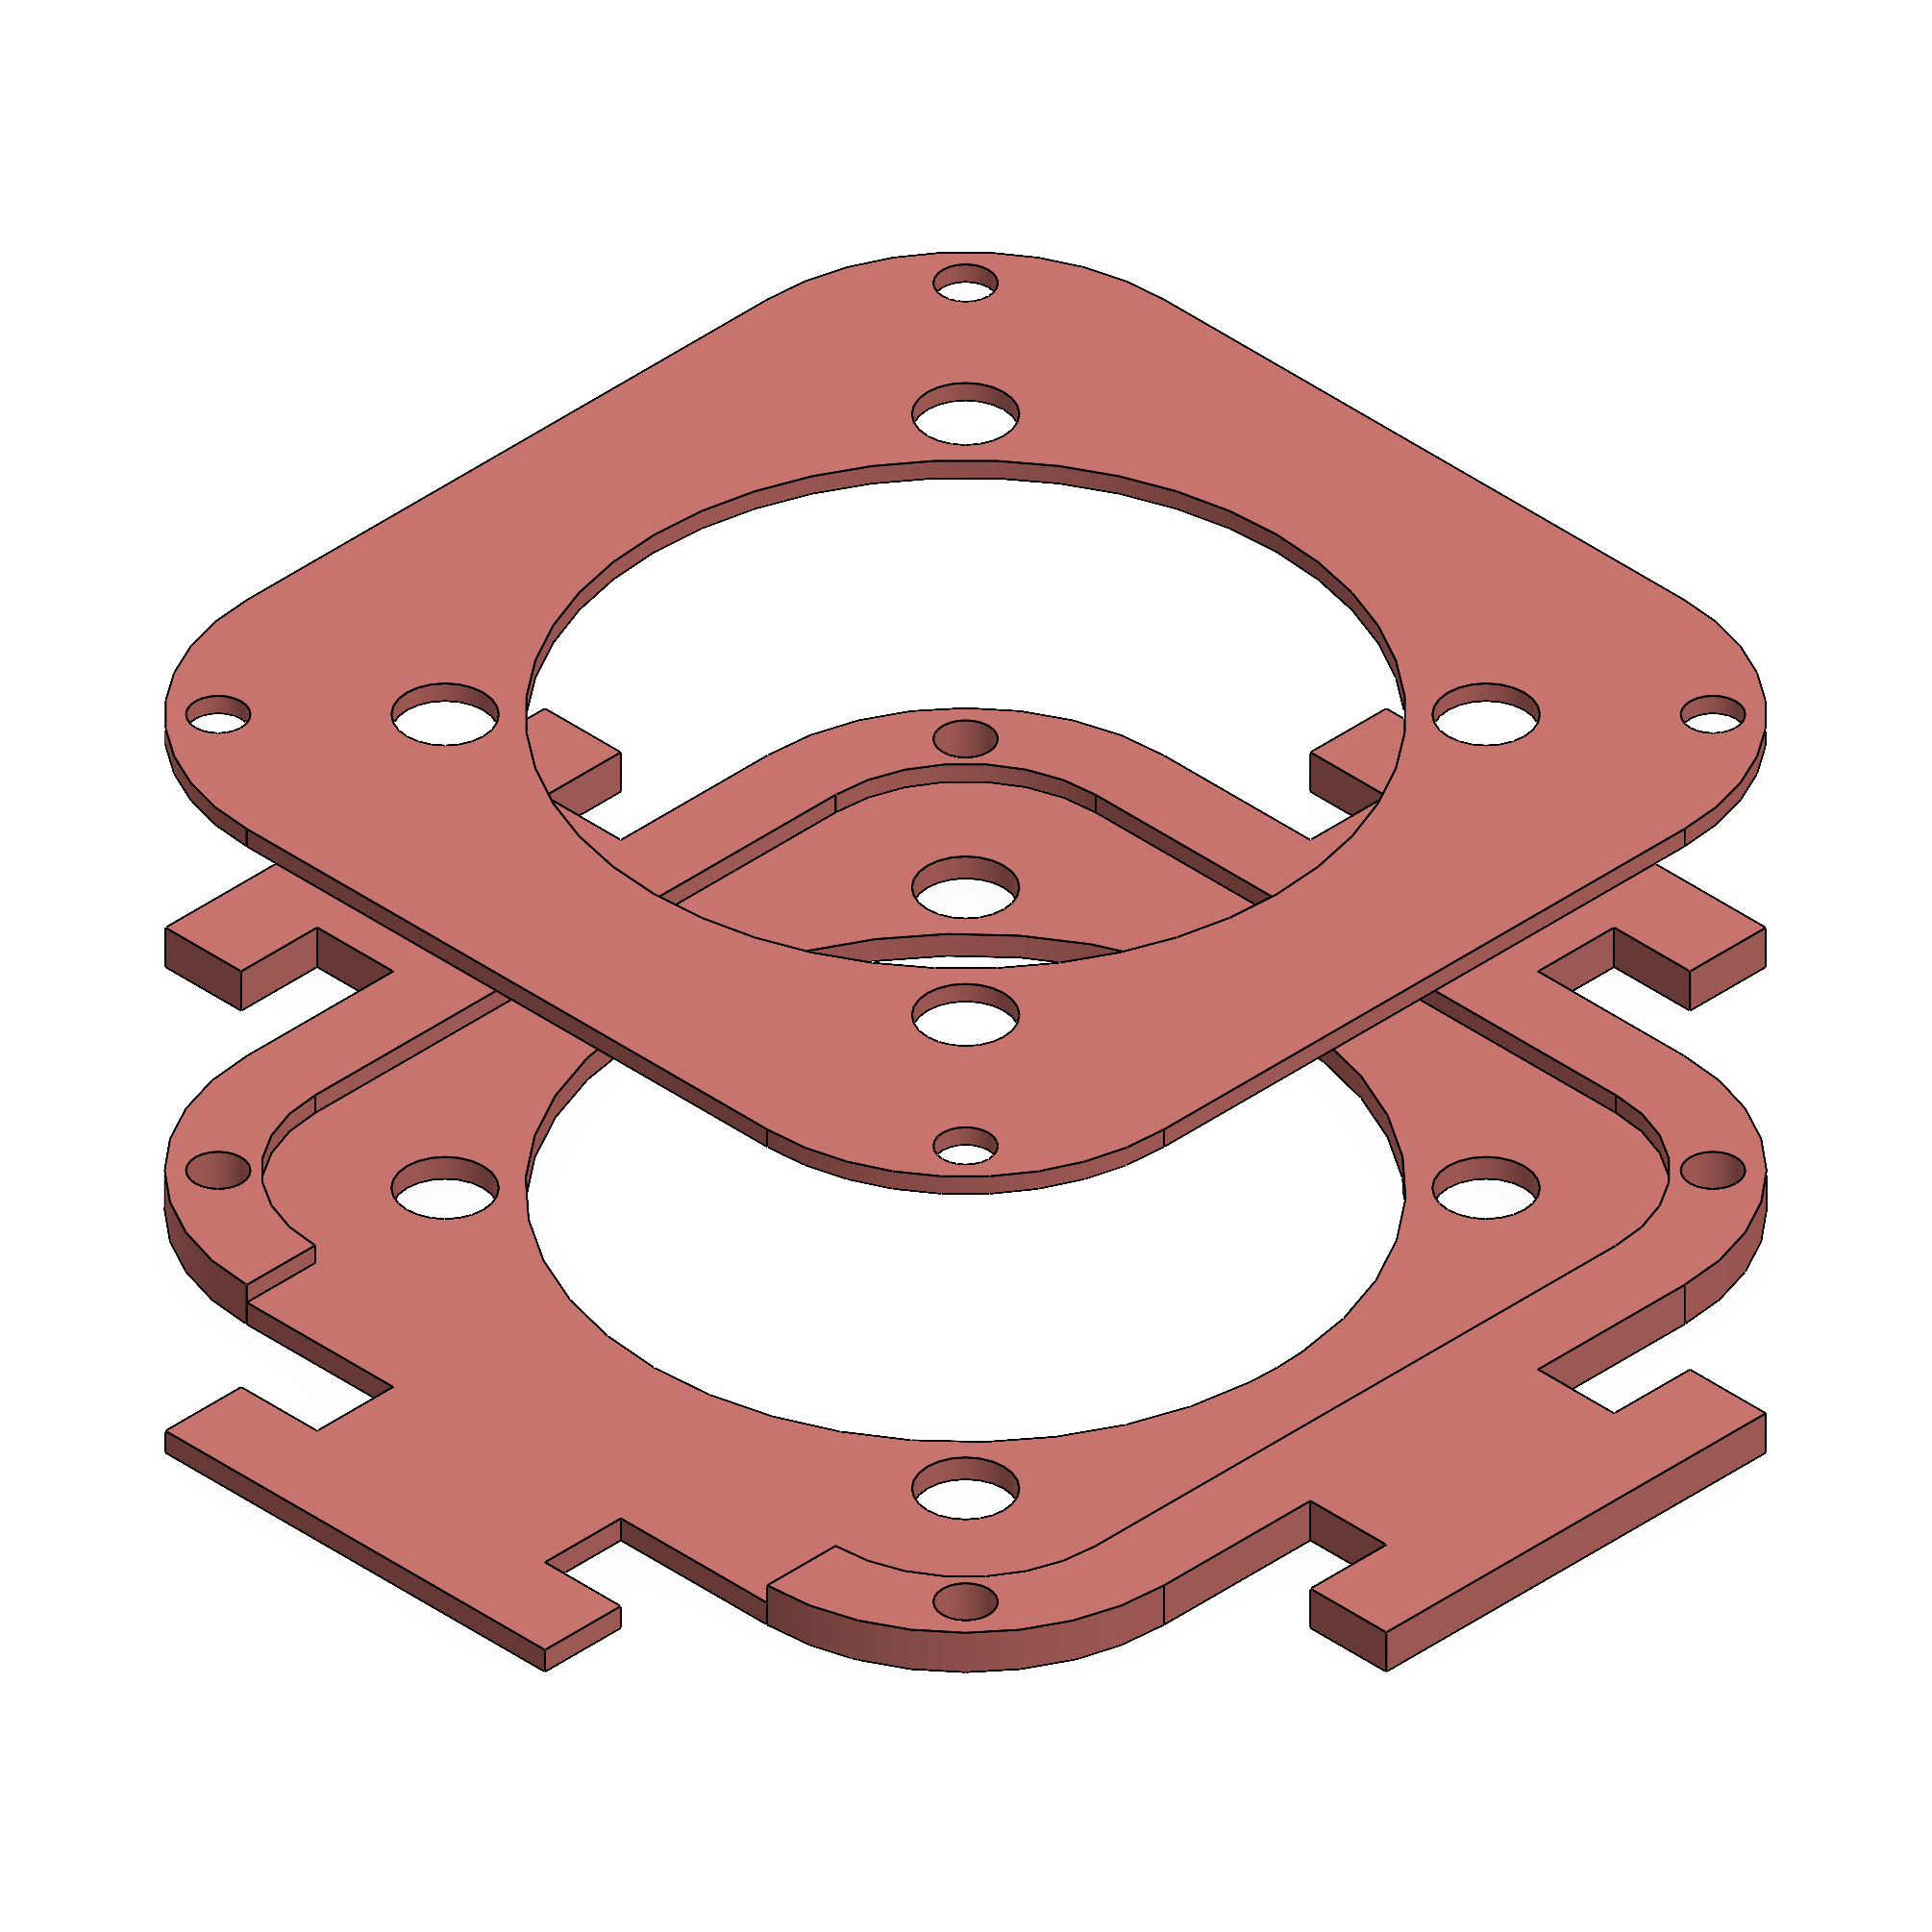
\includegraphics[width=0.15\textwidth]{Figures/coil_trap_expl.png}
            }
        }
        \parbox[b]{0.2\textwidth}{
            \centering
            \usebox{
                \bigimage
            }
        }
        
    \end{subcaptiongroup}
    \caption{Flexible coil trap.}
\end{figure}

This component allows the coil to be kept at an \textbf{optimal distance} from the magnet letting the membrane be \textbf{free to vibrate}.
This prototype resulted in the \textbf{best performances}, the vibrations were more noticeable, the mat was easy to interact with and the device could \textbf{easily flex}.
Nevertheless, we were \textbf{not still satisfied with the strength of the vibrations} it produced, the coil's problems with heating were still present and we had some \textbf{fragility problems} with the membrane and \textbf{flexing issues} with the coil trap. 

\subsection{Experimentation and Evaluation}
During our testing, we measured the \textbf{heating} production of the coil and the \textbf{force produced} by the last prototype membrane.
\subsubsection{Heating Testing}
We powered the coil with an input \textbf{voltage sweep both in DC and AC} conditions while measuring its surface temperature using a \textbf{thermocouple}. The limit of the sweep was chosen to be the maximum voltage that the coil could handle before reaching its \textbf{thermal runaway point}.
\begin{figure}[H]
    \centering
    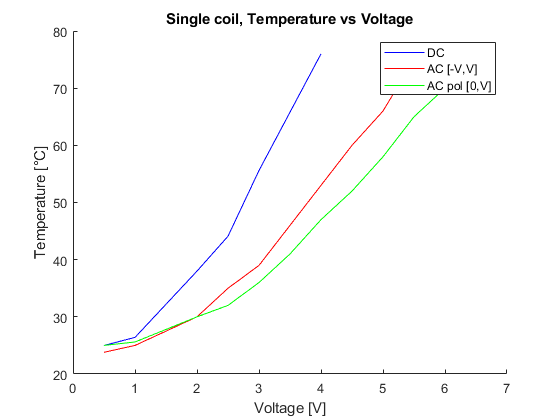
\includegraphics[width = 0.5\linewidth]{Figures/Temp_vs_Volt_1_coil.png}
    \caption{Temperature vs Voltage for one coil.}
    \label{fig: Single_coil_heating_tests}
\end{figure}
As we can observe in figure \ref{fig: Single_coil_heating_tests}, in AC conditions, especially for unipolar signals, the coil can sustain \textbf{higher voltages}; this is because sinusoidal signals have a \textbf{lower RMS} value than DC ones.

\subsubsection{Force Testing}
We measured the force produced by the membrane using an \textbf{ATI TW-Nano17 force sensor}. The prototype's coil was powered with a \textbf{heartbeat-like signal}, as it's a \textbf{very low RMS} signal that allows us to run the coil at \textbf{30V peak voltage}.
This was necessary because the sensor \textbf{sensitivity was too low} to measure the force produced by sinusoidal signals at \textbf{6V}.
\begin{figure}[H]
    \centering
    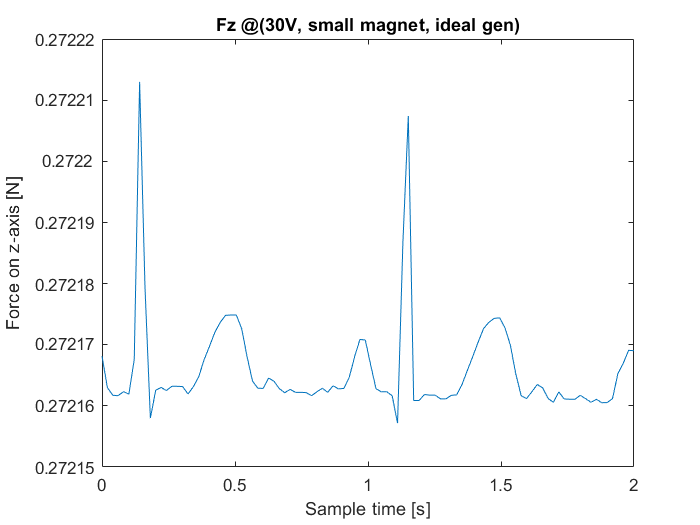
\includegraphics[width = 0.5\linewidth]{Figures/Fz_@30V_small_magn_idealgen.png}
    \caption{Force profile of the generated by the heartbeat signal.}
    \label{fig: Force_profile}
\end{figure}
From figure \ref{fig: Force_profile} we can observe that the membrane produces a \textbf{constant force of about 0.2N}, due to the silicone membrane itself, and the \textbf{net force} produced by the coil at the peak of the signal is in the order of \textbf{$5\cdot10^{-5}$N}.

\section{Introduction}
pizza
Satellite missions and on-orbit services are crucial for various applications, and the integration of AI algorithms has significantly advanced technological capabilities. The rise in in-orbit satellites has increased the complexity of navigation and missions, making AI-driven pose estimation invaluable. The EU-funded EROSS project aims to enhance orbital services, particularly in satellite servicing operations, using robotic space technologies for greater autonomy and safety.\\
AI algorithms, with machine learning capabilities, enable precise processing of onboard sensor data, enhancing accuracy in determining a satellite's position and trajectory. Monocular camera-based pose estimation, a notable AI-driven innovation, reduces hardware complexity and empowers satellites to autonomously process visual data for informed decision-making. This increased autonomy minimizes human intervention, reducing operational costs and enhancing mission efficiency.\\
The thesis focuses on implementing AI algorithms for the rendezvous of a non-collaborative satellite, emphasizing mono camera-based visual pose estimation within the 200-20cm distance range. The project delves into critical aspects of pose estimation throughout the entire rendezvous trajectory, showcasing the transformative potential of AI in space exploration and satellite services.
\section{Algorithms and Methods}
The methodology involves a pipeline that consists in a \textit{Landmark Regression} module for landmarks' location estimation in the image, \textit{Landmark Mapping} module for  landmark 3D position prediction and \textit{CPD} module for pose refinement.
Nine landmarks are manually selected on the satellite CAD model, refined for better recognition.

\begin{figure}[htbp]
\centerline{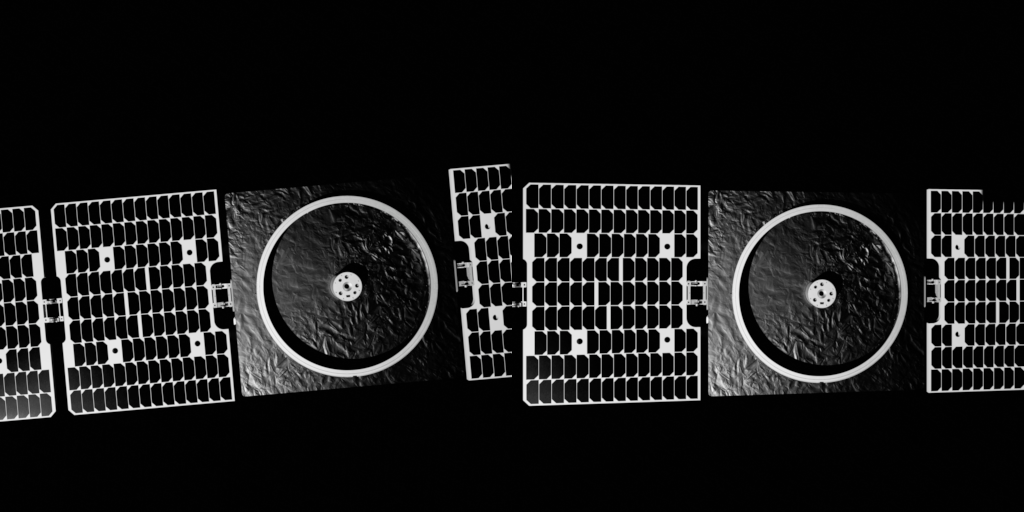
\includegraphics[scale=0.32]{DatabaseExample.png}}
\caption{Sample images from the \textit{TASI EROSS IOD Simulated Dataset N°2}.}
\label{fig}
\end{figure}

\begin{figure*}[t]
\centering
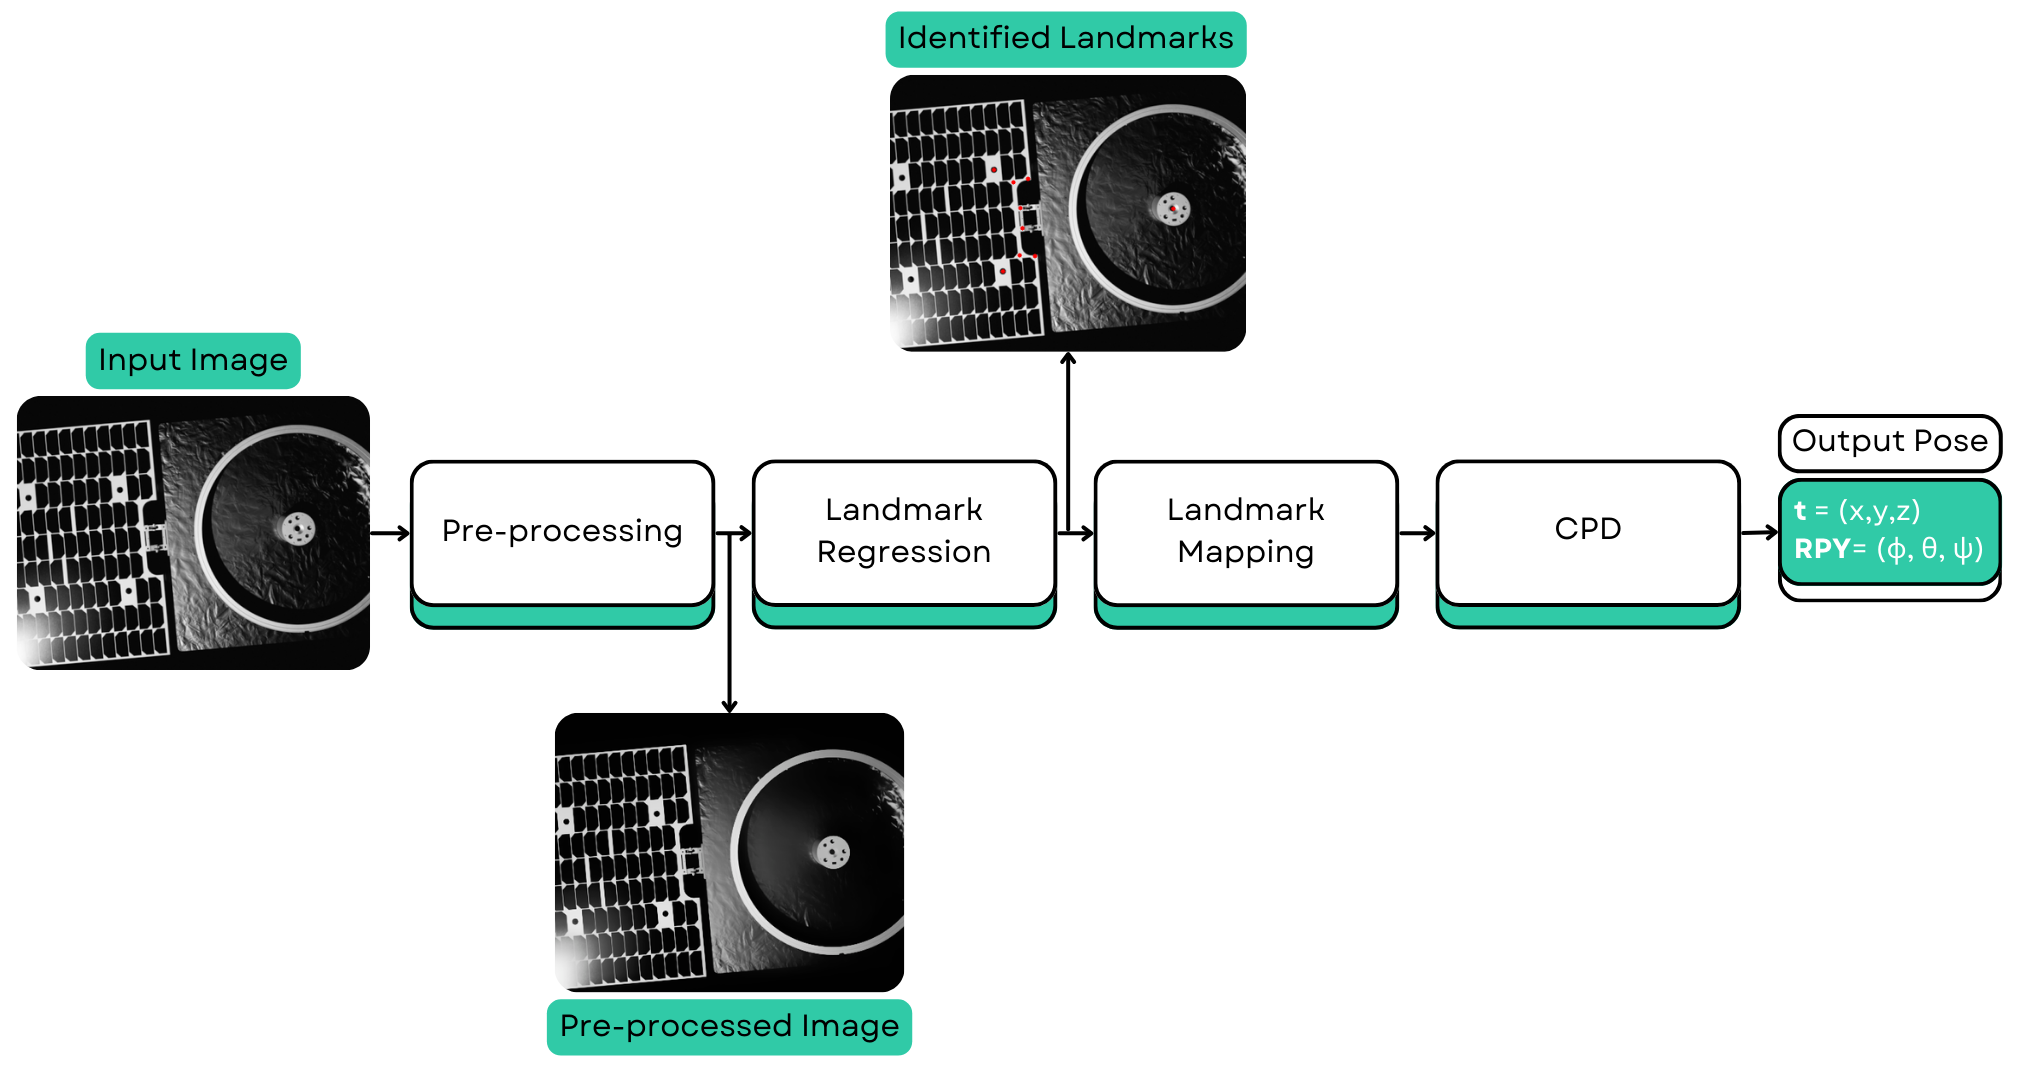
\includegraphics[scale=0.5]{Online Pipeline.png}
\captionof{figure}{Online pipeline of the  satellite pose estimator}
\label{fig}
\end{figure*}

\subsection{Landmark Regression}
The training images are pre-processed and coupled with ground truth 2D landmarks and visibility coefficients.
\[
  v_{i}=\begin{cases}
    1, & \text{if $\textbf{z}_{i}$ is inside image frame}.\\
    0, & \text{otherwise}.
  \end{cases}
\]
The output of the model is a tensor of 9 heatmaps, one for each landmark $h(\textbf{z}_{i}^p)$. The ground truth heatmaps $h(\textbf{z}_{i})$ are generated as 2D normal distributions with mean equal to the ground truth location of each landmark, and standard deviation of 1-pixel.The model is trained from scratch by minimizing the following customized loss:
\[l = \frac{1}{N}\sum_{i=1}^N v_i(h(\textbf{z}_{i}^p) - h(\textbf{z}_{i}))^2\]
The loss function \textit{l} is defined on a single image and in a mini batch \textit{l} is simply averaged. The model is trained in 100 epochs with the \textit{Adam optimizer}.
Landmark positions are selected from heatmaps based on thresholds and variance.
\subsection{Landmark Mapping}
The Landmark Mapping is a neural network designed to estimate the 3D positions of landmarks using their 2D positions, mapping the 2D-3D relation.\\
The network has two hidden layers: the first consists in 128 units and processes the input data learning complex patterns and relationships between the 2D and 3D coordinates. The second hidden layer has 64 units and further refines the features learned in the previous layer. The output layer is responsible for regressing the 3D positions of the landmarks. Each landmark is represented by a 3D coordinate (x, y, z). The output layer produces these 3D coordinates for all the landmarks.\\
The model is trained from scratch by minimizing the following loss:
\[l = \frac{1}{N}\sum_{i=1}^N v_i(\textbf{x}_{i}^p - \textbf{x}_{i})^2\]
where \(\textbf{x}_{i}^p\) represents the 3D position of the \textit{i}-th landmark predicted by the model, while \(\textbf{x}_{i}\) is its ground truth position.\\
As in the previous model, the loss function \textit{l} is defined on a single group of landmarks and in a mini batch it is simply averaged. The model is trained in a maximum of 150 batches with a \textit{Adam optimizer}.\\
In order to improve the accuracy of the algorithm, three models are created, each of them specialized in a specific range of distance from the target.
The training dataset is so split in three subdatasets depending on the distance on the z axis from the satellite with a 100 images superposition per model from each trajectory. The table below shows the specifications of each model.\\
Moreover, in order to prevent overfitting, an Early Stopping algorithm is employed. Overfitting it's where a neural network becomes excessively specialized in training data, hindering generalization, is mitigated by Early Stopping. The algorithm periodically halts the training process to evaluate the network's performance on a validation set, preventing it from becoming too specialized. If consecutive evaluations indicate declining performance (based on a "patience" parameter), it signals potential overfitting. Training ceases at this point, considering the neural network optimized for generalization to new, unseen data, with the parameters finalized for the model.

\subsection{Coherent Point Drift (CPD)}
The \textit{Landmark Mapping} module, predicting each landmark's position independently, introduces misalignment in the 3D point cloud compared to the rigid CAD model reference. To address this and estimate the satellite's 6DOF pose, the Coherent Point Drift technique is employed. Two sets of 3D points are utilized: the "target" represents landmark positions assuming no translation or rotation, and the "source" represents predicted landmark positions. The accuracy of pose estimation is influenced by the number of visible landmarks, reducing as some landmarks are cut from the image frame when the camera approaches the target.
\begin{table*}[ht]
\centering
\scalebox{1.4}{%
\begin{tabular}{l | l l l l | l l | l}

\midrule
Trajectory & $E_{CNN}$ (pxls) & $E_{NN}$ (cm) & $E_T$ (cm)& $E_R$ (°)& $S_T$ & $S_R$ & $S$\\
\midrule
multi-model & 1.38 $\pm$ 0.06 & 1.12 $\pm$ 0.48 & 2.18 $\pm$ 2.09 & 0.046 & 0.0200 & 0.0008 & \textbf{0.0208}\\
\midrule
single-model & 1.38 $\pm$ 0.06 & 0.85 $\pm$ 0.35 & 1.85 $\pm$ 1.19 & 0.058 & 0.0168 & 0.0010 & \textbf{0.0178}\\
\midrule
\end{tabular}}
    \caption{\label{tab1}Results on train set with multi and single model configurations.}
\end{table*}

\begin{table*}[ht]
\centering
\scalebox{1.4}{%
\begin{tabular}{l | l l l l | l l | l}
\midrule
Trajectory & $E_{CNN}$ (pxls) & $E_{NN}$ (cm) & $E_T$ (cm)& $E_R$ (°)& $S_T$ & $S_R$ & $S$\\
\midrule
TRAY\_A & 1.34 $\pm$ 0.05 & 1.08 $\pm$ 0.29 & 2.96 & 0.601 & 0.0238 & 0.0105 & 0.0343\\
TRAY\_B & 1.37 $\pm$ 0.05 & 1.89 $\pm$ 1.60 & 3.62 & 0.281 & 0.0287 & 0.0049 & 0.0336\\
Less\_D\_Tray & 0.00 $\pm$ 0.00 & 1.27 $\pm$ 0.15 & 3.32 & 0.057 & 0.0337 & 0.0010 & 0.0347\\
Difficult\_Tray & 0.00 $\pm$ 0.00 & 5.58 $\pm$ 17.96 & 7.73 & 0.375 & 0.0697 & 0.0066 & 0.0763\\
\midrule
Overall & 1.35 $\pm$ 0.04 & 2.46 $\pm$ 8.38 & 4.41 & 0.328 & 0.0390 & 0.0057 & \textbf{0.0447}\\
\midrule
\end{tabular}}
    
    \caption{\label{tab2}Results on test set with multi-model configuration.}
\end{table*}

\section{Evaluation and Results}
\subsection{Metrics}
The final pose estimation scores are derived based on the errors in rotation and translation. For rotation error ($E_R$), the angular distance between predicted ($q^*$) and ground truth ($q$) unit quaternions is calculated using the Hamilton product:
\[ E_R = 2\cos^{-1}(|z|) \]
where, $z$ is the real part of the Hamilton product between $q^*$ and the conjugate of $q$. Translation error ($E_T$) is the 2-norm of the difference between ground truth (\textbf{t*}) and estimated (\textbf{t}) position vectors:
\[ E_T = \|\textbf{t}^*-\textbf{t}\|_2 \]
The rotation score ($S_R$) equals $E_R$, but in radians, and the translation score ($S_T$) is $E_T$ normalized by ground truth translation:
\[ S_T = \frac{\|\textbf{t}^*-\textbf{t}\|_2}{\|\textbf{t}^*\|_2} \]
The final score ($S$) is the sum of both scores: $S = S_R + S_T$. Iterative assessments after each module execution allow dissecting their impact, providing insights into system dynamics and optimization potential.\\
For the evaluation of the \textit{Landmark Regression} module, the mean error among identified landmarks is computed:
\[ E_{2D} = \frac{\sum_{i=1}^{N} (\textbf{z}^{*}_{i}-\textbf{z}_i)}{N} \]
where $\textbf{z}_{i}^{*}$ and $\textbf{z}_{i}$ are the ground truth and predicted pixel coordinates, respectively, for landmarks with $v=1$ visibility. Overall module error is the L2 norm of the mean error: $E_{CNN} = \|E_{2D}\|_2$.\\
Similar to the previous, the evaluation of the \textit{Landmark Mapping} module is performed using the L2 norm of mean 3D position error for landmarks with $v = 1$ is computed:
\[ E_{3D} = \frac{\sum_{i=1}^{N} (\textbf{x}^{*}_{i}-\textbf{x}_i)}{N} \]
where $\textbf{x}^{*}_{i}$ and $\textbf{x}_i$ are the ground truth and predicted 3D coordinates, respectively. The overall module error is the L2 norm of the mean error: $E_{NN} = \|E_{3D}\|_2$.
\subsection{Experiments}
Two comprehensive experiments assess the system's performance. The initial experiment, conducted on the training dataset, refines parameters through fine-tuning. The \textit{Landmark Regression} module achieves a commendable mean 2D error of $1.38 \pm 0.06$ pixels, showcasing its accuracy. The Landmark Mapping module undergoes testing in both single-model and multi-model configurations to assess its performance across different proximity bands. The multi-model configuration exhibits jumps during transitions between models, impacting the accuracy of 3D position predictions. The single-model configuration, due to more consistency, surpasses the multi-model configuration accuracy in 3D prediction on the training set.\\
The \textit{CPD} module introduces additional error during point set alignment, in particular due to its sensitivity to the number of predicted landmarks. Overall, the system proves its robustness during testing, as 3D errors consistently fall within the stringent EROSS project guidelines of less than 2-5 centimeters. Notably, the multi-model setup shows promise but reveals challenges in the abrupt transitions between models, suggesting the need for a more refined transition logic.\\
In the second experiment, the system is tested on a distinct test dataset. Trajectories \textit{$A$} and \textit{$B$} mirror training images light conditions, while \textit{Less\_Difficult\_Trajectory} and \textit{$Difficult\_Trajectory$} differ significantly, challenging the system's landmark prediction. Given the Landmark Mapping module's sensitivity, evaluation on the latter dataset focuses on Landmark Mapping and CPD modules only, assuming precise landmark predictions (\textit{2D Error = 0}). A nuanced observation reveals an overfitting tendency in the single-model configuration during testing. On the contrary, the multi-model setup displays promising generalization, maintaining proximity in performance between training and testing phases. These results underscore the system's potential for reliable and accurate pose estimation in spaceborne applications, with areas for refinement identified for future optimization. Tables \textbf{\ref{tab1}} and \textbf{\ref{tab2}} show the results on training and test datasets respectively.

\section{Conclusions}
This project introduces a specialized monocular pose estimation framework tailored for spaceborne objects, with a focus on satellite rendezvous maneuvers. Utilizing deep neural networks, it seamlessly integrates feature learning and establishes robust 2D-3D correspondence mapping. The inclusion of HRNet, renowned for high-resolution image representation, enhances pose prediction precision. Additionally, the framework employs geometric optimization techniques, ensuring accurate point set alignment and overall system robustness.
\end{document}
